% chap2.tex (Chapter 2 of the thesis)

\chapter[INCOMPRESSIBLE LINEARIZED SHALLOW ATMOSPHERE MODEL]{INCOMPRESSIBLE LINEARIZED SHALLOW ATMOSPHERE MODEL}
\label{chap:2}
\section{Derivation} \label{sec:incompderiv}
We consider here the basic derivation of the \index{shallow atmosphere!incompressible}incompressible shallow atmosphere equations following the general approach developed in Pedlosky\cite[pages 57--63]{Pedlosky:GFD}. However, as opposed to the rotating cartesian form derived in \cite{Pedlosky:GFD},we initially start in a rotating spherical coordinate system, thus allowing for the curved geometry of the spherical Earth to be appropriately incorporated into the resulting equation set. 

\begin{figure}[htbp]
\psfrag{hd}{\large $h$}
\psfrag{hb}{\large $h_b$}
\psfrag{h}{\large $\bar{h}$}
\psfrag{r=a}{\large $r=a$}
	\centering
		\includegraphics[scale=0.65]{IMAGES/freesurfparams.eps}
	\caption{Free-surface height parameters}
	\label{fig:freesurfparams}
\end{figure}
Commencing the derivation we define \index{$\bar{h}$, free-surface height}$\bar{h}$ as the height of a free-surface surrounding a rotating reference sphere of radius $r=a$ as depicted in Figure~\ref{fig:freesurfparams}. We measure $\bar{h}$ as the radial distance from the level surface $r=a$ of the spherical coordinate system to the free-surface. Additionally, define \index{$h$, free-surface depth}$h$ and $h_b$ as the depth of the fluid and the height of the underlying mountains respectively. The height of the free-surface $\bar{h}$ can be given in terms of the two parameters $h$ and $h_b$ as
\begin{equation}
	\bar{h}=h_b+h.
\end{equation}
Although the generality of this setup affords the representation of a much wider class of problem we will restrict ourselves to the case when there is no underlying mountain specification so that $h_b=0$, leading to
\begin{equation}
	\bar{h}=h.
\end{equation}

Because we are only concerned with incompressible flow in Chapters~\ref{chap:2} and \ref{chap:3}, the equations of motion presented in Chapter~\ref{chap:1} will reduce significantly. In particular, since density $\rho$ is constant the mass equation, \eqref{eq:mass1}, reduces to the form $\nabla\cdot\bol{q}=0$. In addition, we can discard all thermodynamic behaviour, allowing us to remove the \index{energy conservation}energy and \index{ideal gas law}ideal gas equations from the governing system. We also note that, due to the nature of the spherical coordinate system, the vertical coordinate $r$ appears explicitly in the dynamical equations. Holton~\cite[page 24]{Holton:IDM} points out that these \index{curvature terms}curvature terms can be adequately approximated by $r=a$ since the depth of the atmosphere $h$ is assumed to be much smaller than the radius of the earth. Adopting the above approximations and simplifications we obtain the following form for the incompressible dynamical equations.

{\bfseries Mass}
\begin{equation}
a\cos\phi\durd{r}+\dulamd{\lambda}+\frac{\partial}{\partial \, \phi} \left(\uphi\cos\phi \right)= 0, \label{eq:incompmass}
\end{equation}
{\bfseries \boldmath$r$ momentum}
\begin{equation}
\durd{t} +\ur\durd{r}+ \frac{\ulam}{a\cos\phi}\durd{\lambda}+\frac{\uphi}{a}\durd{\phi}-\frac{\ulams+\uphis}{a}-2\Omega\ulam\cos\phi+\frac{1}{\rho}\dpd{r}= -g, \label{eq:incompr}
\end{equation}
{\bfseries \boldmath$\lambda$ momentum}
\begin{multline}
\dulamd{t} +\ur\dulamd{r}+ \frac{\ulam}{a\cos\phi}\dulamd{\lambda}+\frac{\uphi}{a}\dulamd{\phi}+\frac{\ur\ulam-\ulam\uphi\tan\phi}{a}\\+2\Omega(\ur\cos\phi-\uphi\sin\phi)+\frac{1}{a\rho\cos\phi}\dpd{\lambda}= 0, \label{eq:incomplam}
\end{multline}
{\bfseries \boldmath$\phi$ momentum}
\begin{multline}
\duphid{t} +\ur\duphid{r}+ \frac{\ulam}{a\cos\phi}\duphid{\lambda}+\frac{\uphi}{a}\duphid{\phi}+\frac{\ur\uphi+\ulams\tan\phi}{a}\\+2\Omega\ulam\sin\phi+\frac{1}{a\rho}\dpd{\phi}= 0. \label{eq:incompphi}
\end{multline}

The underlying assumption of the \index{shallow atmosphere approximation}shallow atmosphere approximation is that motion mainly occurs in the $\lambda$--$\phi$ plane and less so in the $r$ direction, effectively confining the velocity to predominantly ``horizontal'' motion. Mathematically we can write this statement as
\begin{align}
\ur &\approx O(\epsilon), \label{eq:urapprox}\\
\ulam &\approx O(1), \\
\uphi &\approx O(1),
\end{align}
where $\epsilon$ is a small parameter that reflects the shallowness of the atmosphere relative to the radius of the Earth. In effect, $\epsilon$ might be regarded as the ratio $h/a$ which is typically of order $10^{-3}$ for the Earth. Consider now the implications of this approximation for the $r$ momentum equation \eqref{eq:incompr}. We argue that the total derivative terms $\durd{t}$, $\ur\durd{r}$, $\frac{\ulam}{a\cos\phi}\durd{\lambda}$ and $\frac{\uphi}{a}\durd{\phi}$ are all $O(\epsilon)$ so that the $r$ momentum equation reduces to 
\begin{equation}
-\frac{\ulams+\uphis}{a}-2\Omega\ulam\cos\phi+\frac{1}{\rho}\dpd{r}= -g, \label{eq:incompr1}
\end{equation} where only terms of $O(1)$ have been retained. Finally, we assume that \eqref{eq:incompr1} is dominated by \index{hydrostatic approximation}hydrostatics\footnote{We can be more rigorous and use a \index{scale analysis}scale analysis approach to argue this point. See Pedlosky\cite[page 60]{Pedlosky:GFD} for the finer details of this process}, so that effectively we have
\begin{equation}
\dpd{r}= -\rho g. \label{eq:incompr2}
\end{equation}
Equation (\ref{eq:incompr2}) can be integrated with respect to $r$, \index{pressure!incompressible}yielding
\begin{equation}
p(r,\lambda,\phi,t)=-\rho g r + f(\lambda,\phi,t).
\end{equation}
We fix the value of $f(\lambda,\phi,t)$ by assuming that, on the free-surface $r=a+\bar{h}(\lambda,\phi,t)$, the pressure has the constant value $\po$ so that
\begin{equation}
p(r,\lambda,\phi,t)=\po+\rho g (a+\bar{h}(\lambda,\phi,t)-r). \label{eq:incomppress}
\end{equation}
From (\ref{eq:incomppress}) we immediately obtain
\begin{align}
\dpd{\lambda} & = \rho g \dhd{\lambda}, \\
\dpd{\phi} & = \rho g \dhd{\phi},
\end{align}
implying that the \index{horizontal!pressure gradient}horizontal pressure gradient components are independent of $r$, which in turn implies that the \index{horizontal!acceleration}horizontal accelerations must be $r$-independent also. It is therefore consistent (see Pedlosky~\cite[page 61]{Pedlosky:GFD}) to assume that the horizontal velocity components are also $r$-independent if they are initially so. Thus we must have
\begin{align}
\ulam &\equiv \ulam(\lambda,\phi,t), \\
\uphi &\equiv \uphi(\lambda,\phi,t),
\end{align}
so that, in conjunction with \eqref{eq:urapprox}, the two remaining momentum equations, \eqref{eq:incomplam} and \eqref{eq:incompphi}, taken to $O(1)$ become

{\bfseries \boldmath$\lambda$ momentum}
\begin{equation}
\dulamd{t} + \frac{\ulam}{a\cos\phi}\dulamd{\lambda}+\frac{\uphi}{a}\dulamd{\phi}-\frac{\ulam\uphi\tan\phi}{a}-2\Omega\uphi\sin\phi+\frac{g}{a\rho\cos\phi}\dhd{\lambda}= 0, \label{eq:incomplam1}
\end{equation}
{\bfseries \boldmath$\phi$ momentum}
\begin{equation}
\duphid{t}+ \frac{\ulam}{a\cos\phi}\duphid{\lambda}+\frac{\uphi}{a}\duphid{\phi}+\frac{\ulams\tan\phi}{a}+2\Omega\ulam\sin\phi+\frac{g}{a\rho}\dhd{\phi}= 0. \label{eq:incompphi1}
\end{equation}

We now turn our attention to the mass equation and note that since $\ulam$ and $\uphi$ are $r$-independent we can integrate \eqref{eq:incompmass} with respect to $r$ to give
\begin{equation}
a\cos\phi \, \ur(r,\lambda,\phi,t) = -r\left[\dulamd{\lambda} + \frac{\partial}{\partial \, \phi} \left(\uphi\cos\phi \right) \right] + \tilde{u}_{\scriptscriptstyle r}(\lambda,\phi,t). \label{eq:urgen}
\end{equation}
To determine the nature of $\tilde{u}_{\scriptscriptstyle r}$ we need to examine the boundary conditions on the upper and lower boundaries $r=a+\bar{h}$ and $r=a+h_b$ respectively. On the lower boundary we must have no \index{normal flow}normal flow, otherwise the fluid would penetrate the surface and breach the conservation of mass requirement. Thus on $r=a+h_b$ we must enforce the condition $\bol{q}\cdot\bol{n}=0$ where $\bol{n}$ is a normal to the surface $r=a+h_b$. We can easily show that the normal to the lower boundary is given by
\begin{equation}
\bol{n}=\mbox{\bfseries e}_{r}-\frac{1}{a\cos\phi}\dhbd{\lambda}\mbox{\bfseries e}_{\lambda}-\frac{1}{a}\dhbd{\phi}\mbox{\bfseries e}_{\phi},
\end{equation}
so that
\begin{equation}
\bol{q}\cdot\bol{n}=\ur(a+h_b,\lambda,\phi,t)-\frac{\ulam}{a\cos\phi}\dhbd{\lambda}-\frac{\uphi}{a}\dhbd{\phi}=0.
\end{equation}
Solving for $\ur$ we obtain
\begin{equation}
\ur(a+h_b,\lambda,\phi,t)=\frac{\ulam}{a\cos\phi}\dhbd{\lambda}+\frac{\uphi}{a}\dhbd{\phi}. \label{eq:urhb}
\end{equation}
Substituting \eqref{eq:urhb} into \eqref{eq:urgen} and evaluating at $r=a+h_b$ allows us to solve for $\tilde{u}_{\scriptscriptstyle r}$, which we in turn substitute back into \eqref{eq:urgen}. After simplification we arrive at
\begin{multline}
a\cos\phi \, \ur(r,\lambda,\phi,t) = -r\left[\dulamd{\lambda} + \frac{\partial}{\partial \, \phi} \left(\uphi\cos\phi \right) \right] +\frac{\partial}{\partial \, \lambda}\left(\ulam h_b\right) \\+ \frac{\partial}{\partial \, \phi} \left(\uphi h_b \cos\phi \right). \label{eq:urgen1}
\end{multline}

On the upper boundary we enforce the \index{kinematic condition}kinematic condition 
\begin{equation*}
\frac{\mbox{\footnotesize D\ }}{\mbox{\footnotesize D}t}\left[r-a-\bar{h}(\lambda,\phi,t)\right]=0,
\end{equation*}which states that the fluid can not penetrate the free-surface. Expanding the total derivative and solving for $\ur$ gives
\begin{equation}
\ur(h,\lambda,\phi,t)=\dhd{t}+\frac{\ulam}{a\cos\phi}\dhd{\lambda}+\frac{\uphi}{a}\dhd{\phi}.
\label{eq:urfs}
\end{equation}
Finally, substitution of \eqref{eq:urfs} into \eqref{eq:urgen1} and subsequent simplification yields the incompressible shallow atmosphere mass equation given by
\begin{equation}
a\cos\phi\dhd{t}+\frac{\partial}{\partial \, \lambda}\left(\ulam (\bar{h}-h_b)\right) + \frac{\partial}{\partial \, \phi} \left(\uphi (\bar{h}-h_b) \cos\phi \right)=0. \label{eq:incompmass1}
\end{equation}

We note that since $h=\bar{h}-h_b$, expanding all differential products and writing $f=2\Omega\sin\phi$, we can express the complete \index{conservation equations!dimensional incompressible}dimensional dynamical equations of motion for an incompressible fluid in a rotating spherical coordinate system as 

{\bfseries mass}
\begin{equation}\dhdd{t}+\frac{\ulam}{a\cos\phi}\dhdd{\lambda}+\frac{\uphi}{a}\dhdd{\phi}+\frac{h}{a\cos\phi}\left[\dulamd{\lambda}+\cos\phi\duphid{\phi}-\uphi\sin\phi\right]=0, \label{eq:massincom}
\end{equation}
{\bfseries \boldmath$\lambda$ momentum}
\begin{equation}
\dulamd{t} + \frac{\ulam}{a\cos\phi} \dulamd{\lambda} + \frac{\uphi}{a}\dulamd{\phi} - \left(f + \frac{\ulam}{a}\tan\phi \right)\uphi + \frac{g}{a\cos\phi}\dhdd{\lambda} = 0, \label{eq:lamincom}
\end{equation}
{\bfseries \boldmath$\phi$ momentum}
\begin{equation}\duphid{t}+\frac{\ulam}{a\cos\phi}\duphid{\lambda}+\frac{\uphi}{a}\duphid{\phi}+\left(f+\frac{\ulam}{a}\tan\phi \right)\ulam+\frac{g}{a}\dhdd{\phi}=0. \label{eq:phiincom}
\end{equation}

The above form is that given by Williamson et al.\cite[page 213]{Williamson:STS} as the \index{conservation equations!incompressible advective form}advective form of the shallow atmosphere equations and this is the form we shall subsequently use for all analysis in this chapter.

\section{Progressive-Wave Coordinate Transform} \label{sec:progresswave}
We are interested in solutions to equations \eqref{eq:massincom}, \eqref{eq:lamincom} and \eqref{eq:phiincom} that are of the form of a \index{progressive-wave}progressive-wave with constant angular velocity. Defining \index{$c$, angular wavespeed}$c$ to be an angular wavespeed we now construct a new moving coordinate frame that depends on $\lambda$ and $t$ in the form
\begin{equation}
\eta=\lambda - ct.
\end{equation} 
The effect of the $-ct$ term is to translate any initial wave structure either towards the west ($c<0$) or towards the east ($c>0$) with constant angular speed $c$. Since we have defined a new coordinate system we need to establish how the equations of motion are represented in this new reference frame. Applying the chain rule we can easily show that, for some scalar field $\Psi(\eta,\phi)$,
\begin{align}
\frac{\partial \, \Psi}{\partial \, \lambda} &= \frac{\partial \, \Psi}{\partial \, \eta}\frac{\partial \, \eta}{\partial \, \lambda}=\frac{\partial \, \Psi}{\partial \, \eta},\\[3mm]
\frac{\partial \, \Psi}{\partial \, t} &= \frac{\partial \, \Psi}{\partial \, \eta}\frac{\partial \, \eta}{\partial \, t}=-c\frac{\partial \, \Psi}{\partial \, \eta}.
\end{align}
Using this transformation we can now write equations \eqref{eq:massincom}, \eqref{eq:lamincom} and \eqref{eq:phiincom} as

{\bfseries mass}
\begin{equation}
\left(\frac{\ulam}{a}-c\cos\phi\right)\dhdd{\eta}+\frac{\uphi\cos\phi}{a}\dhdd{\phi}+\frac{h}{a}\left[\dulamd{\eta}+\cos\phi\duphid{\phi}-\uphi\sin\phi\right]=0, \label{eq:massincom1}
\end{equation}
{\bfseries \boldmath$\lambda$ momentum}
\begin{equation}
\left(\frac{\ulam}{a}-c\cos\phi\right)\dulamd{\eta} + \frac{\uphi\cos\phi}{a}\dulamd{\phi} - \left(f\cos\phi + \frac{\ulam}{a}\sin\phi \right)\uphi + \frac{g}{a}\dhdd{\eta} = 0, \label{eq:lamincom1}
\end{equation}
{\bfseries \boldmath$\phi$ momentum}
\begin{equation}
\left(\frac{\ulam}{a}-c\cos\phi\right)\duphid{\eta}+\frac{\uphi\cos\phi}{a}\duphid{\phi}+\left(f\cos\phi+\frac{\ulam}{a}\sin\phi \right)\ulam+\frac{g\cos\phi}{a}\dhdd{\phi}=0, \label{eq:phiincom1}
\end{equation}
where we have multiplied each equation by $\cos\phi$ to remove apparent polar singularities that would otherwise adversely affect numerical computations, and we have also retained the name ``$\lambda$ momentum'' to remind us of the fact that equation \eqref{eq:lamincom1} is essentially still the $\lambda$ component of conservation of momentum despite the transformation to $\eta$.

\section{Non-dimensionalization of the Governing Equations}
In an attempt to generalise the analysis, it is desirable to express the governing partial differential equations in a form that is independent of the specific units used to measure the variables of the problem. For this reason we \index{non-dimensionalization!incompressible equations}non-dimensionalize each of the governing equations to expose the underlying qualitative behaviour. The particular approach adopted here is similar to that used by Klein \cite[page 766]{Klein:AAA} in that we reduce our dimensionless parameters to the set of familiar fluid dynamical parameters comprised of Strouhal number, Froude number and Rossby number. 

First we define the following \index{characteristic scales}characteristic values, for each reference scale contained in the problem, as
\begin{align*}
v_{\mbox{\tiny ref}} & \equiv \mbox{characteristic speed,}\\
h_{\mbox{\tiny ref}} & \equiv \mbox{characteristic free-surface height,} \\
c_{\mbox{\tiny ref}} & \equiv \mbox{characteristic angular velocity.}
\end{align*}
Using these dimensional parameters we now rescale all the field variables to dimensionless form giving
\begin{align}
\hat{u}_{\scriptscriptstyle \lambda}=\frac{\ulam}{v_{\mbox{\tiny ref}}} \quad & \Rightarrow \quad \ulam = v_{\mbox{\tiny ref}} \hat{u}_{\scriptscriptstyle \lambda}, \label{eq:ulamhat}\\
\hat{u}_{\scriptscriptstyle \phi}=\frac{\uphi}{v_{\mbox{\tiny ref}}} \quad & \Rightarrow \quad \ulam = v_{\mbox{\tiny ref}} \hat{u}_{\scriptscriptstyle \phi}, \label{eq:uphihat}\\
\hat{h}=\frac{h}{h_{\mbox{\tiny ref}}} \quad & \Rightarrow \quad h = h_{\mbox{\tiny ref}} \hat{h}, \label{eq:hhat}\\
\hat{c}=\frac{c}{c_{\mbox{\tiny ref}}} \quad & \Rightarrow \quad c = c_{\mbox{\tiny ref}} \hat{c}, \label{eq:chat}
\end{align}
where the hat ($\hat{}$) denotes a dimensionless variable. Substituting equations \eqref{eq:ulamhat}--\eqref{eq:chat} into \eqref{eq:massincom1}, \eqref{eq:lamincom1},  \eqref{eq:phiincom1} and manipulating, we obtain

{\bfseries mass}
\begin{equation}
\left(\hat{u}_{\scriptscriptstyle \lambda}-\frac{c_{\mbox{\tiny ref}}\,a}{v_{\mbox{\tiny ref}}}\,\hat{c}\cos\phi\right)\frac{\partial \, \hat{h}}{\partial \, \eta} + \hat{u}_{\scriptscriptstyle \phi}\cos\phi\frac{\partial \, \hat{h}}{\partial \, \phi}+\hat{h}\left[\frac{\partial \, \hat{u}_{\scriptscriptstyle \lambda}}{\partial \, \eta}+\cos\phi\frac{\partial \, \hat{u}_{\scriptscriptstyle \phi}}{\partial \, \phi}-\hat{u}_{\scriptscriptstyle \phi}\sin\phi\right]=0, \label{eq:massincom1non}
\end{equation}
{\bfseries \boldmath$\lambda$ momentum}
\begin{multline}
\left(\hat{u}_{\scriptscriptstyle \lambda}-\frac{c_{\mbox{\tiny ref}}\,a}{v_{\mbox{\tiny ref}}}\,\hat{c}\cos\phi\right)\frac{\partial \, \hat{u}_{\scriptscriptstyle \lambda}}{\partial \, \eta} + \hat{u}_{\scriptscriptstyle \phi}\cos\phi\frac{\partial \, \hat{u}_{\scriptscriptstyle \lambda}}{\partial \, \phi} - \left(\frac{2\Omega a}{v_{\mbox{\tiny ref}}}\cos\phi + \hat{u}_{\scriptscriptstyle \lambda}\right)\hat{u}_{\scriptscriptstyle \phi}\sin\phi \\+ \frac{g h_{\mbox{\tiny ref}}}{v^2_{\mbox{\tiny ref}}}\frac{\partial \, \hat{h}}{\partial \, \eta} = 0, \label{eq:lamincom1non}
\end{multline}
{\bfseries \boldmath$\phi$ momentum}
\begin{multline}
\left(\hat{u}_{\scriptscriptstyle \lambda}-\frac{c_{\mbox{\tiny ref}}\,a}{v_{\mbox{\tiny ref}}}\,\hat{c}\cos\phi\right)\frac{\partial \, \hat{u}_{\scriptscriptstyle \phi}}{\partial \, \eta} + \hat{u}_{\scriptscriptstyle \phi}\cos\phi\frac{\partial \, \hat{u}_{\scriptscriptstyle \phi}}{\partial \, \phi} + \left(\frac{2 \Omega a}{v_{\mbox{\tiny ref}}}\cos\phi + \hat{u}_{\scriptscriptstyle \lambda} \right)\hat{u}_{\scriptscriptstyle \lambda}\sin\phi \\+ \frac{g h_{\mbox{\tiny ref}}\cos\phi}{v^2_{\mbox{\tiny ref}}}\frac{\partial \, \hat{h}}{\partial \, \phi} = 0, \label{eq:phiincom1non}
\end{multline}
where we have also replaced the \index{Coriolis parameter}Coriolis parameter $f$ by its definition $f=2\Omega\sin\phi$.

Three obvious dimensionless parameter groupings emerge from this process. These are just the familiar flow regime parameters from fluid dynamics given as\index{Strouhal number}\index{Froude number}\index{Rossby number}
\begin{alignat*}{2}
&\mathrm{Sr} = \D \frac{a\,c_{\mbox{\tiny ref}}}{v_{\mbox{\tiny ref}}} &\qquad& \mbox{Strouhal number,} \\[1mm]
&\mathrm{Fr} = \D \frac{v_{\mbox{\tiny ref}}}{\sqrt{gh_{\mbox{\tiny ref}}}} && \mbox{Froude number,} \\[1mm]
&\mathrm{Ro} = \D \frac{v_{\mbox{\tiny ref}}}{2\Omega a} && \mbox{Rossby number.}
\end{alignat*}
Substitution of these parameters into our governing equations yields 

{\bfseries mass}
\begin{equation}
\left(\hat{u}_{\scriptscriptstyle \lambda}-\mathrm{Sr}\,\hat{c}\cos\phi\right)\frac{\partial \, \hat{h}}{\partial \, \eta} + \hat{u}_{\scriptscriptstyle \phi}\cos\phi\frac{\partial \, \hat{h}}{\partial \, \phi}+\hat{h}\left[\frac{\partial \, \hat{u}_{\scriptscriptstyle \lambda}}{\partial \, \eta}+\cos\phi\frac{\partial \, \hat{u}_{\scriptscriptstyle \phi}}{\partial \, \phi}-\hat{u}_{\scriptscriptstyle \phi}\sin\phi\right]=0, \label{eq:massincom2non}
\end{equation}
{\bfseries \boldmath$\lambda$ momentum}
\begin{equation}
\left(\hat{u}_{\scriptscriptstyle \lambda}-\mathrm{Sr}\,\hat{c}\cos\phi\right)\frac{\partial \hat{u}_{\scriptscriptstyle \lambda}}{\partial \eta} + \hat{u}_{\scriptscriptstyle \phi}\cos\phi\frac{\partial \hat{u}_{\scriptscriptstyle \lambda}}{\partial \phi} - \left(\frac{\cos\phi}{\mathrm{Ro}} + \hat{u}_{\scriptscriptstyle \lambda}\right)\hat{u}_{\scriptscriptstyle \phi}\sin\phi + \frac{1}{\mathrm{Fr}^2}\frac{\partial \hat{h}}{\partial \eta} = 0, \label{eq:lamincom2non}
\end{equation}
{\bfseries \boldmath$\phi$ momentum}
\begin{equation}
\left(\hat{u}_{\scriptscriptstyle \lambda}-\mathrm{Sr}\,\hat{c}\cos\phi\right)\frac{\partial \hat{u}_{\scriptscriptstyle \phi}}{\partial \eta} + \hat{u}_{\scriptscriptstyle \phi}\cos\phi\frac{\partial \hat{u}_{\scriptscriptstyle \phi}}{\partial \phi} + \left(\frac{\cos\phi}{\mathrm{Ro}} + \hat{u}_{\scriptscriptstyle \lambda} \right)\hat{u}_{\scriptscriptstyle \lambda}\sin\phi + \frac{\cos\phi}{\mathrm{Fr}^2}\frac{\partial \hat{h}}{\partial \phi} = 0, \label{eq:phiincom2non}
\end{equation}
which is the final form for the \index{shallow atmosphere equations!non-dimensional incompressible}non-dimensional incompressible shallow atmosphere equations on a rotating sphere.
%\pagebreak[4]
\section{Linearization of the Equations}
\subsection{Base Zonal Flow Derivation} \label{sec:incompbase}
As previously discussed in Chapter~\ref{chap:1} it is convenient to consider \index{Rossby wave}Rossby waves as consisting of latitudinal perturbations about an underlying \index{zonal flow}zonal flow structure. Thus it is important to know the exact nature of the zonal flow in order to calculate the resulting perturbations. Following the work of Haurwitz\cite[page 255]{Haurwitz:MAD} we choose the simplest zonal flow in the form of a \index{super rotation}super rotation that only depends on latitude and additionally has $\uphi=0$\footnote{Although all variables are dimensionless, from now on, for the sake of brevity, we drop the hat ($\hat{}$) notation and all variables will be assumed dimensionless unless otherwise stated.}. The form for our zonal flow is then given by
\begin{align}
\ulamz &= \omega\cos\phi, \label{eqn:zlam}\\
\uphiz &= 0,\label{eqn:zphi}\\
\hz &= H(\phi), \label{eqn:zh}
\end{align}
where the parameter \index{$\omega$, zonal angular speed}$\omega$ is the non-dimensional representation of the base angular speed of the flow and the subscript $z$ is used to denote field variables belonging to the zonal flow structure. The problem now reduces to finding the function $H(\phi)$ that makes equations \eqref{eqn:zlam}, \eqref{eqn:zphi} and \eqref{eqn:zh} a solution of equations \eqref{eq:massincom2non}, \eqref{eq:lamincom2non} and \eqref{eq:phiincom2non}. 

Direct substitution reveals that the only equation not identically satisfied by the zonal flow structure is the $\phi$ momentum equation, which yields the ordinary differential equation
\begin{equation}
\frac{d H}{d \phi} = -\omega \mathrm{Fr}^2 \left(\frac{1}{\mathrm{Ro}}+\omega \right)\sin\phi\cos\phi. 
\end{equation}
This integrates easily to give
\begin{equation}
H(\phi) = h_o + \frac{\omega \mathrm{Fr}^2}{2}\left(\frac{1}{\mathrm{Ro}}+\omega \right)\cos^2\!\phi.
\end{equation}
The constant of integration \index{$h_o$, polar free-surface height}$h_o$ can be viewed as the base non-dimensional height of the free-surface at the poles and typically we would choose $h_o=1$ so that the dimensional value of $\hz$ at $\phi=\pm \pi/2$ is $h_{\mbox{\tiny ref}}$. The two parameters $\omega$ and $h_o$ suffice to  specify uniquely any given super rotation and associated total mass, or volume in the incompressible case, of the system. We note here that in order to make comparison between results with differing values of $\omega$ it is necessary to modify the value of $h_o$ so that the total volume of fluid in $a+h_b \le r \le a+\bar{h}$ remains constant. This amounts to solving a cubic equation for $h_o$ once a fixed volume and value for $\omega$ have been decided upon.

In summary, we have shown that a basic zonal flow structure is given by
\begin{align}
\ulamz &= \omega\cos\phi, \label{eqn:zlam1}\\ 
\uphiz &= 0, \label{eqn:zphi1}\\
\hz &= h_o + \frac{\omega \mathrm{Fr}^2}{2}\left(\frac{1}{\mathrm{Ro}}+\omega \right)\cos^2\!\phi. \label{eqn:zh1}
\end{align}

\subsection{Linearization about the Base Zonal Flow}
Given the base zonal flow we now consider $O(\epsilon)$ perturbations about this flow state by constructing the \index{Linearization!incompressible}\index{shallow atmosphere equations!non-dimensional incompressible\\linearized}perturbation expansions
\begin{alignat}{3}
\ulam(\eta,\phi) &= \ulamz &\!&+ \epsilon \ulamp(\eta,\phi) &\!&+ O(\epsilon^2), \label{eq:ulampert}\\
\uphi(\eta,\phi) &= 0 &\!&+ \epsilon \uphip(\eta,\phi) &\!&+ O(\epsilon^2), \label{eq:uphipert}\\
h(\eta,\phi) &= \hz &\!&+ \epsilon \hp(\eta,\phi) &\!&+ O(\epsilon^2). \label{eq:hpert}
\end{alignat}
The perturbation parameter $\epsilon$ is a small quantity that represents the maximum deviation about the zonal flow. It is instructive to think of $\epsilon$ as a wave amplitude in this case, although it must be emphasized that the linearization is only valid for infinitely small amplitude and consequently our results will only be accurate as $\epsilon \rightarrow 0$. Nonetheless we can expect reasonable results for small values of $\epsilon$.

Substituting the perturbation expansions \eqref{eq:ulampert}--\eqref{eq:hpert} into the governing equations \eqref{eq:massincom2non}--\eqref{eq:phiincom2non} leads to the set of partial differential equations given by

{\bfseries mass}
\begin{multline}
\epsilon\left(\ulamz-\mathrm{Sr}\,c\cos\phi\right)\dhpd{\eta} + \epsilon\uphip\cos\phi\frac{d \, \hz}{d \, \phi}\\+\epsilon\hz\left[\dulampd{\eta}+\cos\phi\duphipd{\phi}-\uphip\sin\phi\right]+ O(\epsilon^2)=0, \label{eq:masslin}
\end{multline}
{\bfseries \boldmath$\lambda$ momentum}
\begin{multline}
\epsilon\left(\ulamz-\mathrm{Sr}\,c\cos\phi\right)\dulampd{\eta} + \epsilon\uphip\cos\phi\frac{d \, \ulamz}{d \, \phi} - \epsilon\left(\frac{\cos\phi}{\mathrm{Ro}} + \ulamz \right)\uphip\sin\phi \\ + \frac{1}{\mathrm{Fr}^2}\dhpd{\eta} + O(\epsilon^2) = 0, \label{eq:lamlin}
\end{multline}
{\bfseries \boldmath$\phi$ momentum}
\begin{multline}
\left(\frac{\cos\phi}{\mathrm{Ro}}+\ulamz \right)\ulamz\sin\phi +   \frac{\cos\phi}{\mathrm{Fr}^2}\frac{d\,\hz}{d \, \phi} + \epsilon\left(\ulamz-\mathrm{Sr}\,c\cos\phi\right)\duphipd{\eta} \\+ \epsilon\left(\frac{\cos\phi}{\mathrm{Ro}} + 2\ulamz \right)\ulamp\sin\phi + \frac{\cos\phi}{\mathrm{Fr}^2}\dhpd{\phi} + O(\epsilon^2)= 0. \label{eq:philin}
\end{multline}
The $O(1)$ terms in \eqref{eq:philin} are satisfied identically by the base zonal flow. By putting $\ulamz=\omega\cos\phi$ into the above equations we obtain the $O(\epsilon)$ equations that define the first level of corrections in our perturbation expansions. These equations are

{\bfseries mass}
\begin{equation}
\left(\omega-\mathrm{Sr}\,c\right)\cos\phi\dhpd{\eta} + \uphip\cos\phi\frac{d \, \hz}{d \, \phi}+\hz\left[\dulampd{\eta}+\cos\phi\duphipd{\phi}-\uphip\sin\phi\right]=0, \label{eq:masslin1}
\end{equation}
{\bfseries \boldmath$\lambda$ momentum}
\begin{equation}
\left(\omega-\mathrm{Sr}\,c\right)cos\phi\dulampd{\eta} - \left(\frac{1}{\mathrm{Ro}} + 2\omega\right)\uphip\sin\phi\cos\phi + \frac{1}{\mathrm{Fr}^2}\dhpd{\eta} = 0, \label{eq:lamlin1}
\end{equation}
{\bfseries \boldmath$\phi$ momentum}
\begin{equation}
\left(\omega-\mathrm{Sr}\,c\right)\cos\phi\duphipd{\eta} + \left(\frac{1}{\mathrm{Ro}} + 2\omega \right)\ulamp\sin\phi\cos\phi + \frac{\cos\phi}{\mathrm{Fr}^2}\dhpd{\phi} = 0. \label{eq:philin1}
\end{equation}

The solution of \eqref{eq:masslin1}, \eqref{eq:lamlin1} and \eqref{eq:philin1} is facilitated by noting that we may write each of the $O(\epsilon)$ perturbation terms as the product of a \index{Fourier mode}Fourier mode in $\eta$ with a function of $\phi$. Thus we define
\begin{align}
\ulamp(\eta,\phi) &= \cos(\kappa\eta)\,\Lambda(\phi),\label{eq:ulampcomp}\\
\uphip(\eta,\phi) &= \sin(\kappa\eta)\,\Phi(\phi),\label{eq:uphipcomp}\\
\hp(\eta,\phi) &= \cos(\kappa\eta)\,\mathcal{H}(\phi),\label{eq:hpcomp}
\end{align}
where the \index{parity}parity of the Fourier basis in $\eta$ in each term is chosen to preserve the overall parity of each dynamical equation. Alternatively, it would be possible to interchange the $\sin$ and $\cos$ terms in \eqref{eq:ulampcomp}--\eqref{eq:hpcomp}, with the effect of rotating the solution at $t=0$ by $\pi/\kappa$. Also note that the parameter \index{$\kappa$, longitudinal wavenumber}$\kappa$ has been introduced as a way of specifying the wavenumber of the solution. This is a natural addition to the model since intuitively we would expect that the wavespeed $c$ will depend on the number of equally spaced wavelengths around a latitude circle.

By defining our $O(\epsilon)$ terms according to \eqref{eq:ulampcomp}--\eqref{eq:hpcomp} we can remove the $\eta$ dependence entirely from the partial differential equations, transforming them into a set of ordinary differential and \index{shallow atmosphere equations!non-dimensional incompressible\\linearized}algebraic equations given by

{\bfseries mass}
\begin{multline}
-\kappa\left(\omega-\mathrm{Sr}\,c\right)\cos\phi \, \mathcal{H}(\phi) + \Phi(\phi)\cos\phi\frac{d \, \hz}{d \, \phi}\\+\hz\left[-\kappa\Lambda(\phi)+\cos\phi\frac{d \, \Phi(\phi)}{d\,\phi}-\Phi(\phi)\sin\phi\right]=0, \label{eq:masslin2}
\end{multline}
{\bfseries \boldmath$\lambda$ momentum}
\begin{equation}
-\kappa\left(\omega-\mathrm{Sr}\,c\right)cos\phi \,\Lambda(\phi) - \left(\frac{1}{\mathrm{Ro}} + 2\omega\right)\Phi(\phi)\sin\phi\cos\phi - \frac{\kappa}{\mathrm{Fr}^2}\mathcal{H}(\phi) = 0, \label{eq:lamlin2}
\end{equation}
{\bfseries \boldmath$\phi$ momentum}
\begin{equation}
\kappa\left(\omega-\mathrm{Sr}\,c\right)\Phi(\phi) + \left(\frac{1}{\mathrm{Ro}} + 2\omega \right)\Lambda(\phi)\sin\phi + \frac{1}{\mathrm{Fr}^2}\frac{d \, \mathcal{H}(\phi)}{d\,\phi} = 0. \label{eq:philin2}
\end{equation}

\section{Numerical Solution of the Linearized Equations}
\subsection{Series Representation}
\label{subsec:incomplinser}
The numerical solution of \eqref{eq:masslin2}, \eqref{eq:lamlin2} and \eqref{eq:philin2} can be accomplished by approximating each of $\Lambda(\phi)$, $\Phi(\phi)$ and $\mathcal{H}(\phi)$ with truncated series of \index{basis function}basis functions. As noted by Boyd\cite[page 109]{Boyd:CFSM}, the particular choice of basis function is primarily governed by the geometry involved in the problem. The inherent spherical geometry in the shallow atmosphere problem can be adequately described by using either \index{basis function!spherical harmonics}spherical harmonics or \index{basis function!Fourier}Fourier basis functions, which both cope well with periodic boundary conditions. Although the generally accepted solution approach for problems in spherical geometry, in both meteorological and mathematical circles, is via the spherical harmonics, the sheer simplicity and ease of use of \index{Fourier series}Fourier series is an attractive alternative that, as will be demonstrated shortly, allows for some further analytical manipulation to be carried out, greatly reducing the computational time for any given solution.

The particular form of the Fourier basis components needs careful consideration, primarily  because we can identify key \index{symmetry conditions}symmetry and \index{boundary conditions}boundary conditions that each of the field variables must satisfy. In this study we are only concerned with special types of solutions that obey the following set of conditions:
\begin{itemize}
\item $\ulam$ and $h$ are symmetric with respect to the equator $(\phi=0)$,
\item $\uphi$ is anti-symmetric with respect to the equator,
\item $\ulam$ and $\uphi$ are zero at the poles $(\phi=\pm\pi/2)$,
\item $h$ is constant at the poles.
\end{itemize}
From an analysis of the problem we can show that $\Lambda(\phi)$ and $\mathcal{H}(\phi)$ must be symmetric with respect to the equator whilst $\Phi(\phi)$ must be antisymmetric. This basically says that a northward velocity deflection in the northern hemisphere is equivalent to a southward velocity deflection in the southern hemisphere, whereas the free-surface has the same height at points $(\eta_0,\pm\phi_0)$. From the above list of solution requirements we can also deduce that the $O(\epsilon)$ field variables must all have zero value at the poles. This is necessary because we have \index{convergence of longitude}convergence of lines of longitude at $\phi=\pm\pi/2$ and hence to avoid multi-valued functions for the field variables we require that the perturbations are all zero at the poles\footnote{In general $\mathcal{H}(\phi)$ need only be constant at the poles; however the allowed values for the parameter $\kappa$ effectively force $\mathcal{H}\left(\pm \frac{\pi}{2}\right)=0$.}.

Although the above list of solution requirements might seem, at first glance, to be rather restrictive there is much to be gained by employing such an approach. The main advantage of this formulation is that difficulties at the poles are avoided; this can be a common source of numerical trouble in models that account for the spherical geometry. The \index{pole problem}pole problem amounts to the previously mentioned dilemma of having multi-valued functions defining the flow field and the apparent switching of East to West (or North to South) as one traverses across a pole of the spherical coordinate system. A common approach to navigate this troublesome numerical stumbling block is to introduce new velocity components that are multiplied by Fourier functions that correctly adjust for the parity change on either side of the pole as detailed in Duran\cite[page 207]{Duran:NMW}. In our approach no such adjustments are required since by forcing the flow to have \index{stagnation point}stagnation points at each pole we will never encounter a scenario in which flow with an eastward or northward component suddenly switches to flow having a westward or southward component. Of course, in all realistic global circulation models the handling of the pole problem becomes an integral feature of any time integrating computation since in general stagnation points are not situated at both poles. Nonetheless, the advantages to be had by adopting our approach coupled with the motive of theoretical investigation justify its use.

We are now in a position to construct the series approximations. For now we just state the forms for the $O(\epsilon)$ linear terms, defering the statement of the series for the full nonlinear terms until Chapter~\ref{chap:3} when we approach the solution of the full nonlinear system. The functions that meet our prescribed conditions above can be given by 
\begin{align}
\Lambda(\phi) &= \sum_{n=1}^\infty P_{\kappa,n}\cos\bigl((2n-1)\phi\bigr), \label{eq:Lamseries}\\
\Phi(\phi) &= \sum_{n=1}^\infty Q_{\kappa,n}\sin(2n\phi), \label{eq:Phiseries}\\
\mathcal{H}(\phi) &= \sum_{n=1}^\infty H_{\kappa,n} (-1)^n \left[ \cos(2n\phi)+\cos\bigl(2(n-1)\phi\bigr) \right], \label{eq:Hseries}
\end{align}
where subscript $\kappa$ on each coefficient denotes the longitudinal wave number that we are currently using as defined in equations \eqref{eq:ulampcomp}--\eqref{eq:hpcomp}. 

It is also essential to point out that the particular form of \eqref{eq:Hseries} is due to the process of \index{basis recombination}basis recombination in which we have constructed new basis functions, which are linear combinations of our underlying basis set, that satisfy the required \index{boundary conditions}boundary conditions, as discussed in detail in Boyd\cite[page 112]{Boyd:CFSM}. Basis recombination is needed here since the general representation of $h(\eta,\phi)$ need only be constant at the poles, rather than zero as in the case of the two velocity components $\ulam$ and $\uphi$. Thus the underlying basis set is centered around $\cos(2 n \phi)$ which attains the value of $\pm1$ at the poles. Since we require $\mathcal{H}(\phi)$ to be zero at $\pm \pi/2$ then it becomes the task of basis recombination to satisfy this boundary condition; this is achieved through the particular form of \eqref{eq:Hseries}.

\subsection{Galerkin Method}
\label{subsec:lingalerl}
With the forms for each of our series defined we now tackle the problem of solving for the wavespeed $c$ and associated \index{Fourier coefficients}coefficients $P_{\kappa,n}$, $Q_{\kappa,n}$ and $H_{\kappa,n}$. To do this we exploit the \index{orthogonality}orthogonality properties of the trigonometric functions by requiring that the \index{residual equation}residual equations, obtained after substituting \eqref{eq:Lamseries}--\eqref{eq:Hseries} into \eqref{eq:masslin2}--\eqref{eq:philin2}, be orthogonal to each of our expansion functions. This technique amounts to the standard \index{Galerkin method}Galerkin method which has been used extensively to solve optimization and root finding problems from all areas of mathematics. We now demonstrate the particular application to our problem.

Substitution of \eqref{eq:Lamseries}--\eqref{eq:Hseries} into \eqref{eq:masslin2} yields the algebraic version of the linearized mass equation given by
\begin{align}
-\kappa(\omega &- \mathrm{Sr}\,c) \sum_{n=1}^\infty H_{\kappa,n} (-1)^n \left[ \cos(2n\phi)\cos\phi+\cos\bigl(2(n-1)\phi\bigr)\cos\phi \right] \notag \\
&- \omega \mathrm{Fr}^2 \left( \frac{1}{\mathrm{Ro}}+\omega \right)\sum_{n=1}^\infty Q_{\kappa,n} \sin(2n\phi)\cos^2\phi \sin\phi  \notag \\
&+(h_o + \frac{\omega \mathrm{Fr}^2}{2}\left(\frac{1}{\mathrm{Ro}}+\omega \right)\cos^2\!\phi ) \biggl[-\kappa\sum_{n=1}^\infty P_{\kappa,n}\cos\bigl((2n-1)\phi\bigr) \notag \\
&+\sum_{n=1}^\infty Q_{\kappa,n}2n\cos(2n\phi)\cos\phi-\sum_{n=1}^\infty Q_{\kappa,n}\sin(2n\phi)\sin\phi\biggr]=0. \label{eq:masssub1}
\end{align}
We can show that general terms of \eqref{eq:masssub1} take the form $\cos((2l-1)\phi)$, for $l=0,1,2,\ldots$, so these become our base expansion functions and the \index{orthogonality}orthogonality condition is now equivalent to multiplying \eqref{eq:masssub1} by $\cos((2l-1)\phi)$, integrating from $-\pi/2\le\phi\le\pi/2$ and equating to zero. Performing these operations we have
\begin{align}
-\kappa(\omega &- \mathrm{Sr}\,c) \sum_{n=1}^\infty H_{\kappa,n} (-1)^n \int_{-\frac{\pi}{2}}^{\frac{\pi}{2}} \cos(2n\phi)\cos\phi\cos\bigl((2l-1)\phi\bigr)\,d\phi \notag \\
&+\kappa(\omega - \mathrm{Sr}\,c) \sum_{n=1}^\infty H_{\kappa,n} (-1)^n \int_{-\frac{\pi}{2}}^{\frac{\pi}{2}}\cos\bigl(2(n-1)\phi\bigr)\cos\phi\cos\bigl((2l-1)\phi\bigr)\,d\phi \notag \\
&- \omega \mathrm{Fr}^2 \left( \frac{1}{\mathrm{Ro}}+\omega \right)\sum_{n=1}^\infty Q_{\kappa,n} \int_{-\frac{\pi}{2}}^{\frac{\pi}{2}}\sin(2n\phi)\cos^2\!\phi \sin\phi\cos\bigl((2l-1)\phi\bigr)\,d\phi  \notag \\
&-h_o \kappa \sum_{n=1}^\infty P_{\kappa,n}\int_{-\frac{\pi}{2}}^{\frac{\pi}{2}} \cos\bigl((2n-1)\phi\bigr)\cos\bigl((2l-1)\phi\bigr)\,d\phi \notag\\
&+2h_o\sum_{n=1}^\infty n Q_{\kappa,n} \int_{-\frac{\pi}{2}}^{\frac{\pi}{2}} \cos(2n\phi)\cos\phi\cos\bigl((2l-1)\phi\bigr)\,d\phi \notag \\
&-h_o\sum_{n=1}^\infty Q_{\kappa,n} \int_{-\frac{\pi}{2}}^{\frac{\pi}{2}} \sin(2n\phi)\sin\phi \cos\bigl((2l-1)\phi\bigr)\,d\phi  \notag \\
&-\frac{\kappa \omega \mathrm{Fr}^2}{2}\left(\frac{1}{\mathrm{Ro}}+\omega \right)\sum_{n=1}^\infty P_{\kappa,n} \int_{-\frac{\pi}{2}}^{\frac{\pi}{2}} \cos\bigl((2n-1)\phi\bigr)\cos^2\!\phi \cos\bigl((2l-1)\phi\bigr)\,d\phi \notag \\
&+\omega \mathrm{Fr}^2\left(\frac{1}{\mathrm{Ro}}+\omega \right)\sum_{n=1}^\infty n Q_{\kappa,n} \int_{-\frac{\pi}{2}}^{\frac{\pi}{2}} \cos(2n\phi)\cos^3\!\phi \cos\bigl((2l-1)\phi\bigr)\,d\phi \notag \\
&-\frac{\omega \mathrm{Fr}^2}{2}\left(\frac{1}{\mathrm{Ro}}+\omega \right)\sum_{n=1}^\infty Q_{\kappa,n} \int_{-\frac{\pi}{2}}^{\frac{\pi}{2}} \sin(2n\phi)\sin\phi\cos^2\!\phi \cos\bigl((2l-1)\phi\bigr)\,d\phi=0. \label{eq:massint1}
\end{align}

All of the integrals in \eqref{eq:massint1} can be rewritten by using trigonometric identities to express the integrands in terms of products of two of the base expansion functions. As an example, we consider the first integral in \eqref{eq:massint1} and note that the integrand may be written, with the aid of the identity $\cos(A-B)+\cos(A+B)=2\cos A\cos B$, as
\begin{align}
\cos(2n\phi)\cos\phi\cos\bigl((2l-1)\phi\bigr)&=\frac{1}{2}\left[\cos\bigl((2n+1)\phi\bigr)+\cos\bigl((2n-1)\phi\bigr)\right]\cos\bigl((2l-1)\phi\bigr) \notag\\
&=\frac{1}{2}\cos\bigl((2n+1)\phi\bigr)\cos\bigl((2l-1)\phi\bigr) \notag \\
&{} \quad\, +\frac{1}{2}\cos\bigl((2n-1)\phi\bigr)\cos\bigl((2l-1)\phi\bigr). \label{eq:trigident}
\end{align}
In addition we then, if required, \index{index shifting}shift the index on the resulting integrands so that every integral in equation \eqref{eq:massint1} is transformed to one of the form
\begin{align}
I_{\text{o}}&=\int_{-\frac{\pi}{2}}^{\frac{\pi}{2}} \cos\bigl((2n-1)\phi\bigr) \cos\bigl((2l-1)\phi\bigr)\,d\phi, \label{eq:orthocond} \\
&=\begin{cases}
\frac{\displaystyle \pi}{2}& \text{if $n=l$, ($n=0$ and $l=1$) or ($n=1$ and $l=0$}),\\[2mm]
0& \text{otherwise},
\end{cases} \label{eq:orthog}
\end{align}where the {\itshape o} subscript denotes an integral obtained by using orthogonality. 

Applying trigonometric identities, similar to that used in \eqref{eq:trigident}, to all the integrals in \eqref{eq:massint1} and then shifting the indices on those terms that require it we obtain
\begin{align}
-&\frac{\kappa}{2}(\omega-\mathrm{Sr}\,c)\sum_{n=0}^\infty H_{\kappa,n+1} (-1)^{n+1} I_{\text{o}} 
-\kappa(\omega-\mathrm{Sr}\,c)\sum_{n=1}^\infty H_{\kappa,n} (-1)^n I_{\text{o}} \notag \\
&-\frac{\kappa}{2}(\omega-\mathrm{Sr}\,c)\sum_{n=2}^\infty H_{\kappa,n-1} (-1)^{n-1} I_{\text{o}} -\frac{\omega \mathrm{Fr}^2}{8}\left( \frac{1}{\mathrm{Ro}}+\omega \right) \left[\sum_{n=0}^\infty Q_{\kappa,n+1}I_{\text{o}}\right. \notag \\
&\quad+\left.\sum_{n=1}^\infty Q_{\kappa,n}I_{\text{o}}-\sum_{n=2}^\infty Q_{\kappa,n-1}I_{\text{o}}-\sum_{n=3}^\infty Q_{\kappa,n-2}I_{\text{o}}\right]-h_o\kappa\sum_{n=1}^\infty P_{\kappa,n}I_{\text{o}} \notag \\
&+h_o\sum_{n=1}^\infty n Q_{\kappa,n}I_{\text{o}}+h_o\sum_{n=2}^\infty (n-1)Q_{\kappa,n-1}I_{\text{o}}-\frac{h_o}{2}\sum_{n=1}^\infty Q_{\kappa,n}I_{\text{o}}+\frac{h_o}{2}\sum_{n=2}^\infty Q_{\kappa,n-1}I_{\text{o}} \notag \\
&-\frac{\kappa \omega \mathrm{Fr}^2}{8}\left( \frac{1}{\mathrm{Ro}}+\omega \right)\left[ \sum_{n=0}^\infty P_{\kappa,n+1}I_{\text{o}}+2\sum_{n=1}^\infty P_{\kappa,n}I_{\text{o}}+\sum_{n=2}^\infty P_{\kappa,n-1}I_{\text{o}} \right] \notag \\
&-\frac{\omega \mathrm{Fr}^2}{16}\left( \frac{1}{\mathrm{Ro}}+\omega \right)\left[ \sum_{n=0}^\infty Q_{\kappa,n+1}I_{\text{o}} + \sum_{n=1}^\infty Q_{\kappa,n}I_{\text{o}}-\sum_{n=2}^\infty Q_{\kappa,n-1}I_{\text{o}}-\sum_{n=3}^\infty Q_{\kappa,n-2}I_{\text{o}}\right] \notag \\
&+\frac{\omega \mathrm{Fr}^2}{8}\left( \frac{1}{\mathrm{Ro}}+\omega \right)\left[\sum_{n=0}^\infty (n+1)Q_{\kappa,n+1}I_{\text{o}} + 3\sum_{n=1}^\infty nQ_{\kappa,n}I_{\text{o}} \right. \notag \\
&\quad+\left.3\sum_{n=2}^\infty (n-1)Q_{\kappa,n-1}I_{\text{o}}+\sum_{n=3}^\infty (n-2)Q_{\kappa,n-2}I_{\text{o}}\right] =0. \label{eq:shifted}
\end{align}

Each integral $I_{\text{o}}$ in \eqref{eq:shifted} is now in the standard form given by \eqref{eq:orthocond} allowing us to use the orthogonality conditions given in \eqref{eq:orthog} to extract a set of \index{orthogonality!algebraic equations}algebraic equations for each value of the integer $l$. Letting $l=1$ and performing some algebraic manipulations we arrive at
\begin{align}
&\left[-\kappa h_o -\frac{3\kappa \omega \mathrm{Fr}^2}{8}\left( \frac{1}{\mathrm{Ro}}+\omega \right)\right] P_{\kappa,1} -\frac{\kappa \omega \mathrm{Fr}^2}{8}\left( \frac{1}{\mathrm{Ro}}+\omega \right)P_{\kappa,2} \notag \\
&\quad+ \left[\frac{h_o}{2} +\frac{\omega \mathrm{Fr}^2}{8}\left( \frac{1}{\mathrm{Ro}}+\omega \right)\right] Q_{\kappa,1} + \frac{\omega \mathrm{Fr}^2}{16}\left( \frac{1}{\mathrm{Ro}}+\omega \right) Q_{\kappa,2} \notag \\
&\quad+\frac{3\kappa \omega}{2}H_{\kappa,1}-\frac{\kappa \omega}{2}H_{\kappa,2}=c\left[\frac{3\kappa \mathrm{Sr}}{2}H_{\kappa,1}-\frac{\kappa \mathrm{Sr}}{2}H_{\kappa,2} \right],\label{eq:massl0}
\end{align}
where we have taken the terms involving the wavespeed $c$ to the right hand side in preparation for the numerical solution method, to be discussed shortly. We also note that letting $l=1$ is equivalent to letting $l=0$ since the nature of the orthogonality of $\cos\bigl((2n-1)\phi\bigr)\cos\bigl((2l-1)\phi\bigr)$ is the same in both cases.

In a similar vein we now consider the case when $l=2$, leading to
\begin{align}
&-\frac{\kappa \omega \mathrm{Fr}^2}{8}\left( \frac{1}{\mathrm{Ro}}+\omega \right)P_{\kappa,1} + \left[-\kappa h_o -\frac{\kappa \omega \mathrm{Fr}^2}{4}\left( \frac{1}{\mathrm{Ro}}+\omega \right)\right] P_{\kappa,2} \notag \\
&\quad-\frac{\kappa \omega \mathrm{Fr}^2}{8}\left( \frac{1}{\mathrm{Ro}}+\omega \right)P_{\kappa,3} + \left[\frac{3 h_o}{2} +\frac{9\omega \mathrm{Fr}^2}{16}\left( \frac{1}{\mathrm{Ro}}+\omega \right)\right] Q_{\kappa,1} \notag \\
&\quad+\left[\frac{3 h_o}{2} +\frac{9\omega \mathrm{Fr}^2}{16}\left( \frac{1}{\mathrm{Ro}}+\omega \right)\right] Q_{\kappa,2} +\frac{3\omega \mathrm{Fr}^2}{16}\left( \frac{1}{\mathrm{Ro}}+\omega \right) Q_{\kappa,3} \notag \\
&\quad+\frac{\kappa \omega}{2}H_{\kappa,1}-\kappa \omega H_{\kappa,2}+\frac{\kappa \omega}{2}H_{\kappa,3}=c\left[\frac{\kappa \mathrm{Sr}}{2} H_{\kappa,1}-\kappa \mathrm{Sr} H_{\kappa,2}+\frac{\kappa \mathrm{Sr}}{2} H_{\kappa,3} \right]. \label{eq:massl2}
\end{align}

Finally, the cases for $l\ge3$ are given by
\begin{align}
&-\frac{\kappa \omega \mathrm{Fr}^2}{8}\left( \frac{1}{\mathrm{Ro}}+\omega \right)P_{\kappa,l-1} + \left[-\kappa h_o -\frac{\kappa \omega \mathrm{Fr}^2}{4}\left( \frac{1}{\mathrm{Ro}}+\omega \right)\right] P_{\kappa,l} \notag \\
&\quad-\frac{\kappa \omega \mathrm{Fr}^2}{8}\left( \frac{1}{\mathrm{Ro}}+\omega \right)P_{\kappa,l+1} +\frac{\omega (2l-1)\mathrm{Fr}^2}{16}\left( \frac{1}{\mathrm{Ro}}+\omega \right)Q_{\kappa,l-2} \notag\\
&\quad+ \left[\frac{(2l-1) h_o}{2} +\frac{3(2l-1)\omega \mathrm{Fr}^2}{16}\left( \frac{1}{\mathrm{Ro}}+\omega \right)\right] Q_{\kappa,l-1} \notag \\
&\quad+\left[\frac{(2l-1) h_o}{2}+\frac{3(2l-1)\omega \mathrm{Fr}^2}{16}\left( \frac{1}{\mathrm{Ro}}+\omega \right)\right] Q_{\kappa,l} \notag \\
&\quad+\frac{\omega(2l-1) \mathrm{Fr}^2}{16}\left( \frac{1}{\mathrm{Ro}}+\omega \right) Q_{\kappa,l+1}+\frac{\kappa \omega (-1)^l}{2}H_{\kappa,l-1}-\kappa \omega (-1)^l H_{\kappa,l}\notag \\
&\quad+\frac{\kappa \omega (-1)^l}{2}H_{\kappa,l+1}=c\left[\frac{\kappa \mathrm{Sr}(-1)^l}{2} H_{\kappa,l-1}-\kappa \mathrm{Sr}(-1)^l H_{\kappa,l}+\frac{\kappa \mathrm{Sr}(-1)^l}{2} H_{\kappa,l+1} \right]. \label{eq:massl3p}
\end{align}
Equations \eqref{eq:massl0}, \eqref{eq:massl2} and \eqref{eq:massl3p} constitute an infinite set of algebraic relationships representing mass conservation that must be satisfied for a solution to be valid. In a similar manner we can derive equivalent algebraic relationships from both the $\lambda$ and $\phi$ momentum equations, \eqref{eq:lamlin2} and \eqref{eq:philin2}, by substituting our series expressions for the $O(\epsilon)$ field variables and using orthogonality to generate the required equations.

From the $\lambda$ momentum equation we have: For $l=0$,
\begin{equation}
-\frac{\kappa \omega}{2} P_{\kappa,1}-\frac{1}{4}\left(\frac{1}{\mathrm{Ro}}+\omega \right) Q_{\kappa,1} + \frac{\kappa}{\mathrm{Fr}^2} H_{\kappa,1} = c\left[-\frac{\kappa \mathrm{Sr}}{2} P_{\kappa,1} \right], \label{eq:laml0}
\end{equation}
for $l=1$,
\begin{multline}
-\frac{\kappa \omega}{2} P_{\kappa,1}-\frac{\kappa \omega}{2} P_{\kappa,2}-\frac{1}{4}\left(\frac{1}{\mathrm{Ro}}+\omega \right) Q_{\kappa,2} + \frac{\kappa}{\mathrm{Fr}^2} H_{\kappa,1}- \frac{\kappa}{\mathrm{Fr}^2} H_{\kappa,2} \\
= c\left[-\frac{\kappa \mathrm{Sr}}{2} P_{\kappa,1} -\frac{\kappa \mathrm{Sr}}{2} P_{\kappa,2}\right] \label{eq:laml1}
\end{multline}
and for $l\ge2$,
\begin{multline}
-\frac{\kappa \omega}{2} P_{\kappa,l}-\frac{\kappa \omega}{2} P_{\kappa,l+1}+\frac{1}{4}\left(\frac{1}{\mathrm{Ro}}+\omega \right) Q_{\kappa,l-1}-\frac{1}{4}\left(\frac{1}{\mathrm{Ro}}+\omega \right) Q_{\kappa,l+1} \\- \frac{\kappa(-1)^l}{\mathrm{Fr}^2} H_{\kappa,l}+ \frac{\kappa(-1)^l}{\mathrm{Fr}^2} H_{\kappa,l+1}
= c\left[-\frac{\kappa \mathrm{Sr}}{2} P_{\kappa,l} -\frac{\kappa \mathrm{Sr}}{2} P_{\kappa,l+1}\right]. \label{eq:laml2p}
\end{multline}
Similarly from the $\phi$ momentum equation we have, for $l\ge1$,
\begin{multline}
\frac{1}{2}\left(\frac{1}{\mathrm{Ro}}+\omega \right)P_{\kappa,l}-\frac{1}{2}\left(\frac{1}{\mathrm{Ro}}+\omega \right)P_{\kappa,l+1}+\kappa \omega Q_{\kappa,l} + \frac{2l(-1)^{l+1}}{\mathrm{Fr}^2} H_{\kappa,l}\\- \frac{2l(-1)^{l+1}}{\mathrm{Fr}^2} H_{\kappa,l+1}=c\left[\kappa \mathrm{Sr} Q_{\kappa,l}\right]. \label{eq:phil1p}
\end{multline}

\subsection{Truncation and Generalised Eigenvalue Formulation}
The set of algebraic equations \eqref{eq:massl0}--\eqref{eq:phil1p} represent an infinite \index{linear system!infinite}linear system in the form of a \index{generalised eigenvalue problem}generalised eigenvalue problem. In order to perform any numerical work it is essential to truncate this system to some finite size. Let $N\in\mathbf{\mathbb{N}}$ define an integer \index{Fourier series!truncation}truncation level so that our infinite series \eqref{eq:Lamseries}--\eqref{eq:Hseries} are now truncated to sums over the finite domain $1\le n \le N$ for $n\in\mathbf{\mathbb{N}}$. Since we have three field variables to solve for we will have a total of $3N$ unknown coefficients, requiring $3N$ equations to close the system. 

Our choice of equations from the set \eqref{eq:massl0}--\eqref{eq:phil1p} is rather intuitive and obvious in that we use exactly $N$ equations from each physical law. To elucidate this process we note that the orthogonalised version of the mass equation consists of two base equations, \eqref{eq:massl0} and \eqref{eq:massl2}, and an infinite series of equations in the form of a \index{recurrence relation}recurrence relation \eqref{eq:massl3p}. To obtain exactly $N$ equations from this set we retain the first two equations along with $N-2$ from the recurrence relation so that the limit on $l$ in \eqref{eq:massl3p} is now $l=3,4,5,\ldots,N$. Note that when $l=N$ we make reference to the coefficients $P_{\kappa,N+1}$, $Q_{\kappa,N+1}$ and $H_{\kappa,N+1}$ but these and higher-order coefficients are ignored in the truncation of the series \eqref{eq:Lamseries}--\eqref{eq:Hseries}. Thus when $l=N$ we have the modified version of \eqref{eq:massl3p} given by
\begin{align}
&-\frac{\kappa \omega \mathrm{Fr}^2}{8}\left( \frac{1}{\mathrm{Ro}}+\omega \right)P_{\kappa,N-1} + \left[-\kappa h_o -\frac{\kappa \omega \mathrm{Fr}^2}{4}\left( \frac{1}{\mathrm{Ro}}+\omega \right)\right] P_{\kappa,N} \notag \\
&\quad+\frac{\omega (2N-1)\mathrm{Fr}^2}{16}\left( \frac{1}{\mathrm{Ro}}+\omega \right)Q_{\kappa,N-2} \notag\\
&\quad+ \left[\frac{(2N-1) h_o}{2} +\frac{3(2N-1)\omega \mathrm{Fr}^2}{16}\left( \frac{1}{\mathrm{Ro}}+\omega \right)\right] Q_{\kappa,N-1} \notag \\
&\quad+\left[\frac{(2N-1) h_o}{2}+\frac{3(2N-1)\omega \mathrm{Fr}^2}{16}\left( \frac{1}{\mathrm{Ro}}+\omega \right)\right] Q_{\kappa,N} \notag \\
&\quad+\frac{\kappa \omega (-1)^N}{2}H_{\kappa,N-1}-\kappa \omega (-1)^N H_{\kappa,N}\notag \\
&\quad=c\left[\frac{\kappa \mathrm{Sr}(-1)^N}{2} H_{\kappa,N-1}-\kappa \mathrm{Sr}(-1)^N H_{\kappa,N} \right]. \label{eq:masslN}
\end{align}

In a similar way we note that the orthogonalised version of the $\lambda$ momentum equation also consists of two base equations, \eqref{eq:laml0} and \eqref{eq:laml1}, and an infinite \index{recurrence relation}recurrence set \eqref{eq:laml2p}. Again, to obtain exactly $N$ equations from this set we retain the first two equations and $N-2$ equations from the recurrence relation so that the limit on $l$ in \eqref{eq:laml2p} is $l=2,3,4,\ldots,N-1$. Since the maximum coefficient index is $N$, occuring when $l=N-1$, we only index into coefficients that are members of the truncated set so no special treatment, analogous to that used to obtain \eqref{eq:masslN} above, is required in this case.

The orthogonalised version of the $\phi$ momentum equation consists of one infinite recurrence relation which we truncate to $N$ equations by imposing the limit $l=1,2,3,\ldots,N$ on $l$ in \eqref{eq:phil1p}. When $l=N$ it is again necessary to ignore $P_{\kappa,N+1}$, $Q_{\kappa,N+1}$ and $H_{\kappa,N+1}$ and higher-order coefficients, giving a special form of \eqref{eq:phil1p} for this case. The result is
\begin{equation}
\frac{1}{2}\left(\frac{1}{\mathrm{Ro}}+\omega \right)P_{\kappa,N}+\kappa \omega Q_{\kappa,N} + \frac{2N(-1)^{N+1}}{\mathrm{Fr}^2} H_{\kappa,N}=c\left[\kappa \mathrm{Sr} Q_{\kappa,N}\right]. \label{eq:philN}
\end{equation}

The set of equations \eqref{eq:massl0}--\eqref{eq:phil1p}, coupled with the two special terminating conditions \eqref{eq:masslN} and \eqref{eq:philN}, constitute a complete \index{generalised eigenvalue problem!truncated}generalised eigenvalue problem of the form
\begin{equation*}
A \bol{x}=cB\bol{x},
\end{equation*}
where $A$ and $B$ are matrices corresponding to the left and right hand sides of each of our algebraic equations. The \index{eigenvalue}eigenvalue $c$ is precisely the wavespeed for our progressive Rossby waves, and vector $\bol{x}$ is the \index{eigenvector}eigenvector of unknown linearized coefficients which we define as
\begin{equation}
\bol{x}=\begin{pmatrix}  H_{\kappa,1} \\ \vdots \\ H_{\kappa,N} \\P_{\kappa,1} \\ \vdots \\ P_{\kappa,N} \\ Q_{\kappa,1} \\ \vdots \\ Q_{\kappa,N}
\end{pmatrix}.
\end{equation}
We note that the general structure of both $A$ and $B$ is that of a \index{diagonal matrix}banded diagonal matrix with $A$ also containing banded sub and super diagonal components . In particular we note that diagonal matrix $B$ consists of non-zero elements along the main diagonal and thus will be invertible, implying that we will always be able to find solutions of our generalised eigensystem. 

\section{Solution and Results}
\subsection{Parameters and Constants}
Now that the linearized problem has been formulated, all that remains is to specify the particular values for the dimensionless parameters in the model and to solve the resulting system. Although this analysis is not specific to a given sphere size or mass it seems reasonable to use parameters that closely approximate those of the Earth so that direct comparison can be made between the present model and other published results. \index{parameter specification}With this in mind we adopt the following values for the sphere specific parameters:
\begin{align}
a&=6.37122\times10^6\text{m},\\
\Omega&=\frac{2 \pi}{24\times3600}\approx7.272\times10^{-5}\,\text{s}^{-1},\\
g&=9.80616\,\text{m}\,\text{s}^{-2}.
\end{align}
Additionally we define each characteristic reference scale as
\begin{align}
v_{\mbox{\tiny ref}}&=40\,\text{m}\,\text{s}^{-1},\\
h_{\mbox{\tiny ref}}&=8.0\times10^{3}\text{m},\\
c_{\mbox{\tiny ref}}&=\frac{\Omega}{30}\approx2.4241\times10^{-6}\,\text{s}^{-1}.
\end{align}
Note that whilst the values for $h_{\mbox{\tiny ref}}$ and $c_{\mbox{\tiny ref}}$ seem ``reasonable'' with reference to the Earth, one should not be surprised at the rather large value of $v_{\mbox{\tiny ref}}$. Normally, to compute velocities similar to those observed locally on the surface of the Earth one must include the effects of friction and the planetary boundary layer in the problem. Neglecting these terms, as we have done is this analysis,  will always result in higher than observed surface velocities, which accounts for the larger than normal choice of $v_{\mbox{\tiny ref}}$.

With the specification of the above parameters we can now calculate estimates for the \index{Strouhal number}Strouhal, \index{Froude number}Froude and \index{Rossby number}Rossby numbers. These are given by
\begin{align}
&\mathrm{Sr} = \D \frac{a\,c_{\mbox{\tiny ref}}}{v_{\mbox{\tiny ref}}} \approx3.8611 \times 10^{-1},\\
&\mathrm{Fr} = \D \frac{v_{\mbox{\tiny ref}}}{\sqrt{gh_{\mbox{\tiny ref}}}} \approx1.4281 \times 10^{-1},\\
&\mathrm{Ro} = \D \frac{v_{\mbox{\tiny ref}}}{2\Omega a} \approx 4.3166 \times 10^{-2}.
\end{align}
The small value of $\mathrm{Ro}$ is in agreement with the definition of \index{large-scale flow}large-scale flow defined by Pedlosky\cite[pages 2--3]{Pedlosky:GFD} so that we can expect the Earth's rotation to be an influential factor determining the nature of any calculated solution. This is precisely the kind of behaviour we seek since we require flows in which the dominant driving force sustaining any initial perturbation is highly dependent on the large scale nature of the flow, as first demonstrated by Rossby\cite{Rossby:RBV}.

For the dimensionless zonal flow parameters we choose values that are consistent with those documented in the test set of Williamson~et~al.\cite{Williamson:STS}. The equivalent non-dimensional values for $h_o$ and $\omega$ are
\begin{align}
h_o&=1,\\
\omega&\approx1.25.
\end{align}
The value of 1 for $h_o$ is consistent with our previous statement about the dimensional value of $h$ at $\phi=\pm \pi/2$ being $h_{\mbox{\tiny ref}}$, and the particular value of $\omega$ above is obtained by noting that Williamson~et~al. use a dimensional value for $\omega$ of $7.848\times10^{-6}\,\text{s}^{-1}$, a value first introduced by Phillips\cite{Phillips:NIP} in 1956 when he successfully integrated the primitive equations of atmospheric flow. In order to convert this to a dimensionless number it is necessary to multiply by the radius of the Earth and divide by the reference velocity scale so that
\begin{equation}
\omega=\frac{7.848\times10^{-6}a}{v_{\mbox{\tiny ref}}}\approx1.25.
\label{eq:wnondim}
\end{equation}
Although \eqref{eq:wnondim} is only a single value of the dimensionless zonal flow angular speed, the analysis presented here permits a wide variety of values for $\omega$.  Nevertheless, the value given by \eqref{eq:wnondim} facilitates comparison with other published literature, such as Williamson~et~al.~\cite{Williamson:STS}. In the next section we will consider the solution for values of $\omega$ over a wide range of allowable values including the specific value above, anticipating the strong dependence of the nonlinear solution on $\omega$ which will be discussed in Chapter~\ref{chap:3}.

\subsection[Results for $\kappa=3,4$ and 5]{Results for \boldmath$\kappa=3,4$ and 5}
\label{sec:incomlinresul}
The solution of the \index{generalised eigenvalue problem!solution of}generalised eigenvalue problem was achieved by implementing a MATLAB script that assembled the left and right hand side matrices and then solved the resulting system by using the inbuilt routine \texttt{\textbf{eig(A,B)}} to find the eigenvalues and corresponding eigenvectors. Various truncation levels were chosen to check \index{convergence}convergence of the algorithm and in all cases rapid convergence was observed for increasing $N$. Typically a truncation value of $N=10$ was all that was required to establish the solution to 4 or 5 significant figures and a truncation level of $N=100$ could almost be deemed excessive if not for the very small computational times involved; approximately 3 seconds was required to compute all 300 eigenvalue--eigenvector pairs when $N=100$, on an AMD Athlon(tm) XP 1800+ processor clocked at 1.54~GHz with 512~MB of physical memory clocked at 266~MHz.

Tables \ref{tab:incompconverg3}, \ref{tab:incompconverg4} and \ref{tab:incompconverg5} illustrate this rapid convergence for $\kappa=3$, 4 and 5 respectively.
\begin{table}[htbp]
	\centering
		\begin{tabular}{|c|r|r|r|r|c|} \hline
		N&\multicolumn{1}{|c|}{3}&\multicolumn{1}{|c|}{5}&\multicolumn{1}{|c|}{10}&
		\multicolumn{1}{|c|}{100}&$O(\text{Coeff}_{100})$ \\
		\hline
		$H_{3,1}$ &-4.6628E-02& -4.4294E-02&-4.4505E-02& -4.4507E-02&\\
		$H_{3,2}$ &-2.4242E-02&-2.2917E-02&-2.3022E-02&-2.3023E-02&1.0E-09 \\
		$H_{3,3}$ &9.3363E-03&1.1141E-02&1.1256E-02&1.1258E-02& \\ \hline
		$P_{3,1}$ &-1.7968E-01&-1.7071E-01&-1.7152E-01&-1.7153E-01& \\
		$P_{3,2}$ &-6.5140E-01&-6.1965E-01&-6.2262E-01&-6.2265E-01&1.0E-06\\
		$P_{3,3}$ &-2.1733E-01&-1.7497E-01&-1.7495E-01&-1.7494E-01& \\ \hline
		$Q_{3,1}$ &-1.0157E+00&-9.6486E-01&-9.6945E-01&-9.6948E-01& \\
		$Q_{3,2}$ &-2.6718E-01&-2.5611E-01&-2.5740E-01&-2.5741E-01&1.0E-07\\
		$Q_{3,3}$ &1.1171E-02&5.1071E-02&5.2422E-02&5.2437E-02& \\ \hline
		$c$ &-4.1957E-02&-4.1805E-02&-4.1805E-02&-4.1805E-02&- \\
		\hline			
		\end{tabular}
	\caption{Convergence of incompressible wavespeed and first three coefficients in each series for increasing N, $\kappa=3$.}
	\label{tab:incompconverg3}
\end{table}
The final column in each table gives the order of the last coefficient in each series when $N=100$ and provides evidence for the accuracy of the solution since in each case the coefficients are observed to drop off reasonably fast and in the case of $\kappa=4$ we have accuracy to very high precision. The particular scaling for the coefficients is arbitrary and has been chosen to match the equivalent Rossby-Haurwitz wave as specified in \cite{Williamson:STS}, to be explained in the next section. Note also that convergence of the eigenvalue is obtained with smaller truncation than that required for corresponding accuracy in the coefficients, providing confidence in the accuracy of the wavespeeds calculated. 
\begin{table}[htbp]
	\centering
		\begin{tabular}{|c|r|r|r|r|c|} \hline
		N&\multicolumn{1}{|c|}{3}&\multicolumn{1}{|c|}{5}&\multicolumn{1}{|c|}{10}&
		\multicolumn{1}{|c|}{100}&$O(\text{Coeff}_{100})$ \\
		\hline
		$H_{4,1}$ &-3.0905E-02 & -2.9884E-02&-2.9888E-02& -2.9888E-02&\\
		$H_{4,2}$ &-1.2042E-02&-1.1779E-02&-1.1781E-02&-1.1781E-02&1.0E-17 \\
		$H_{4,3}$ &1.1248E-02&1.1718E-02&1.1719E-02&1.1719E-02& \\ \hline
		$P_{4,1}$ &-1.0749E-01&-1.0392E-01&-1.0393E-01&-1.0393E-01& \\
		$P_{4,2}$ &-5.0323E-01&-4.8531E-01&-4.8537E-01&-4.8537E-01&1.0E-15\\
		$P_{4,3}$ &-2.5965E-01&-2.3376E-01&-2.3379E-01&-2.3379E-01& \\ \hline
		$Q_{4,1}$ &-9.1506E-01&-8.8487E-01&-8.8498E-01&-8.8498E-01& \\
		$Q_{4,2}$ &-4.0863E-01&-3.9154E-01&-3.9158E-01&-3.9158E-01&1.0E-15\\
		$Q_{4,3}$ &6.5631E-03&3.0816E-02&3.0825E-02&3.0825E-02& \\ \hline
		$c$ &9.5282E-01&9.5522E-01&9.5522E-01&9.5522E-01&- \\
		\hline			
		\end{tabular}
	\caption{Convergence of incompressible wavespeed and first three coefficients in each series for increasing N, $\kappa=4$.}
	\label{tab:incompconverg4}
\end{table}
\begin{table}[htbp]
	\centering
		\begin{tabular}{|c|r|r|r|r|c|} \hline
		N&\multicolumn{1}{|c|}{3}&\multicolumn{1}{|c|}{5}&\multicolumn{1}{|c|}{10}&
		\multicolumn{1}{|c|}{100}&$O(\text{Coeff}_{100})$ \\
		\hline
		$H_{5,1}$ &-2.1197E-02& -2.1753E-02&-2.1665E-02&-2.1665E-02&\\
		$H_{5,2}$ &-6.2402E-03&-6.2807E-03&-6.2548E-03&-6.2548E-03&1.0E-12 \\
		$H_{5,3}$ &1.0452E-02&1.0325E-02&1.0284E-02&1.0284E-02& \\ \hline
		$P_{5,1}$ &-6.8086E-02&-6.9875E-02&-6.9590E-02&-6.9590E-02& \\
		$P_{5,2}$ &-3.7993E-01&-3.9110E-01&-3.8951E-01&-3.8951E-01&1.0E-10\\
		$P_{5,3}$ &-2.3940E-01&-2.5611E-01&-2.5506E-01&-2.5506E-01& \\ \hline
		$Q_{5,1}$ &-7.9287E-01&-8.1367E-01&-8.1037E-01&-8.1036E-01& \\
		$Q_{5,2}$ &-4.5979E-01&-4.7615E-01&-4.7422E-01&-4.7422E-01&1.0E-10\\
		$Q_{5,3}$ &-8.0105E-04&-1.7789E-02&-1.7677E-02&-1.7677E-02& \\ \hline
		$c$ &1.5811E+00&1.5791E+00&1.5791E+00&1.5791E+00&- \\
		\hline			
		\end{tabular}
	\caption{Convergence of incompressible wavespeed and first three coefficients in each series for increasing N, $\kappa=5$.}
	\label{tab:incompconverg5}
\end{table}

As already stated, we need not only consider the value of $\omega$ as used by Williamson et al. Indeed it is important to investigate the behaviour of the solution over a wide range of valid $\omega$ values. We now define precisely what we mean by \index{valid zonal flow value}``valid''. It was noted in Section~ \ref{sec:incompbase} that, to make comparison between solutions with different values of $\omega$ it is essential to make sure that the volume\footnote{In general we need to consider the total mass of the fluid; however the incompressibility condition means that \index{volume conservation}volume conservation is equivalent to mass conservation in this case} of fluid between the surface of the sphere and the free-surface is the same in each case. Since the linearized waves are effectively perturbations of the zonal flow, we need only match the volumes for each underlying zonal flow state because in the limit as $\epsilon\to0$ the flow will reduce to this form.

To perform this analysis then, we need to agree on a volume that will remain constant throughout all the calculations. For now, let this volume be denoted by \index{$V_b$, base volume}$V_b$ where the subscript $b$ represents the base volume. $V_b$ can be any positive volume we decide upon as long as it remains small compared to the volume of the sphere so that the shallow atmosphere approximation is not violated. Generally one would choose $V_b$ to be the volume of the atmosphere without any super rotation so that the free-surface has uniform height 1 everywhere and the volume is just given by the region bounded inside the two concentric spheres of radii $\hat{a}$ and $\hat{a}+1$, so that
\begin{equation*}
V_b=\frac{4\pi}{3}+4\pi \hat{a}(1+\hat{a}).
\end{equation*}
Here we have denoted the dimensionless form of the sphere's radius by $\hat{a}$, which is just the dimensional value divided by the reference height of the free-surface. 

With a base volume decided upon we now ask the question; if the value of $\omega$ changes how must the value of $h_o$ change to ensure that the volume remains constant? To answer this question we note that for the general zonal flow described in \eqref{eqn:zh1}, the \index{$V_z$, zonal flow volume}volume is given by
\begin{align}
V_z&=\int\limits_0^{2\pi} \int\limits_{-\pi/2}^{\pi/2} \int\limits_{\hat{a}}^{\hat{a}+h_z(\phi)} r^2 \cos\phi\,dr d\phi d\eta \notag  \\
&=\frac{4\pi}{3} \int\limits_0^{\pi/2} \left[ h_z^3+3h_z \hat{a}(h_z+\hat{a}) \right]\cos\phi \,d\phi. \label{eq:volz}
\end{align}
The \index{volume matching condition}volume matching condition states that $V_z-V_b=0$, thus
substituting \eqref{eqn:zh1} into \eqref{eq:volz} and performing algebraic manipulations leads to a cubic equation for $h_o$ of the form
\begin{multline}
\frac{4 \pi}{3}h_o^3+\left( \frac{8\pi A}{3}+4 \pi \hat{a} \right)h_o^2 +\left( \frac{32\pi A^2}{15}+\frac{16\pi \hat{a} A}{3}+4 \pi \hat{a}^2 \right)h_o\\
+\left( \frac{64\pi A^3}{105}+\frac{32\pi \hat{a} A^2}{15}+\frac{8\pi \hat{a}^2 A}{3}-V_b \right)=0 \label{eq:hocubic}
\end{multline}
where $A=\frac{\omega \mathrm{Fr}^2}{2}\left(\frac{1}{\mathrm{Ro}}+\omega \right)$. Once $\omega$ is fixed, which in turn fixes the coefficients in \eqref{eq:hocubic}, we can solve for $h_o$ using any appropriate method we choose, be it analytical or numerical. For the present purposes, the formula for the one real root of a cubic equation was used to solve for $h_o$, as taken from Abramowitz \& Stegun\cite{Abramowitz:HMF}.

In general we may choose any value for $\omega$; however for \eqref{eq:hocubic} to have non-negative solutions we can show that there is an upper limit on the value that $\omega$ can take, since the polar height $h_o$ must decrease as the super-rotation rate increases, when volume remains fixed. The limiting upper value on $\omega$, denoted $\omega_u$, will be encountered once the solution of \eqref{eq:hocubic} returns $h_o=0$. Similarly we can also argue for a lower limit of $\omega=0$ since by definition of the linearization process we need to have a base zonal flow to perturb about, which can only occur for non-zero $\omega$. In conclusion we must restrict our investigation to the \index{valid zonal flow value}valid range of values from $0<\omega \le \omega_u$. 

With a volume matching method agreed upon we can now investigate the behaviour of the eigenvalues for constant volume and varying $\omega$. For this analysis we present results only for the case $\kappa=4$ since similar behaviour is observed when $\kappa=3$ or 5. For a given truncation $N$ we will have a total of $3N$ eigenvalues computed. Figure \ref{fig:wvcincompfull} shows the 15 calculated eigenvalues when $N=5$ for valid values of parameter $\omega$. Although the truncation level is quite low here it is useful to observe what is going on at this level since we can clearly distinguish between successive \index{eigenspectrum!incompressible}eigenvalues in the spectrum. 
\begin{figure}[htbp]
\psfrag{Zonal flow angular speed, w}{\scriptsize Zonal flow angular speed, $\omega$}
\psfrag{Wave speed, c}{\scriptsize Wavespeed, $c$}
%\psfrag{R-H solutions}{\scriptsize R-H solutions}
	\centering
		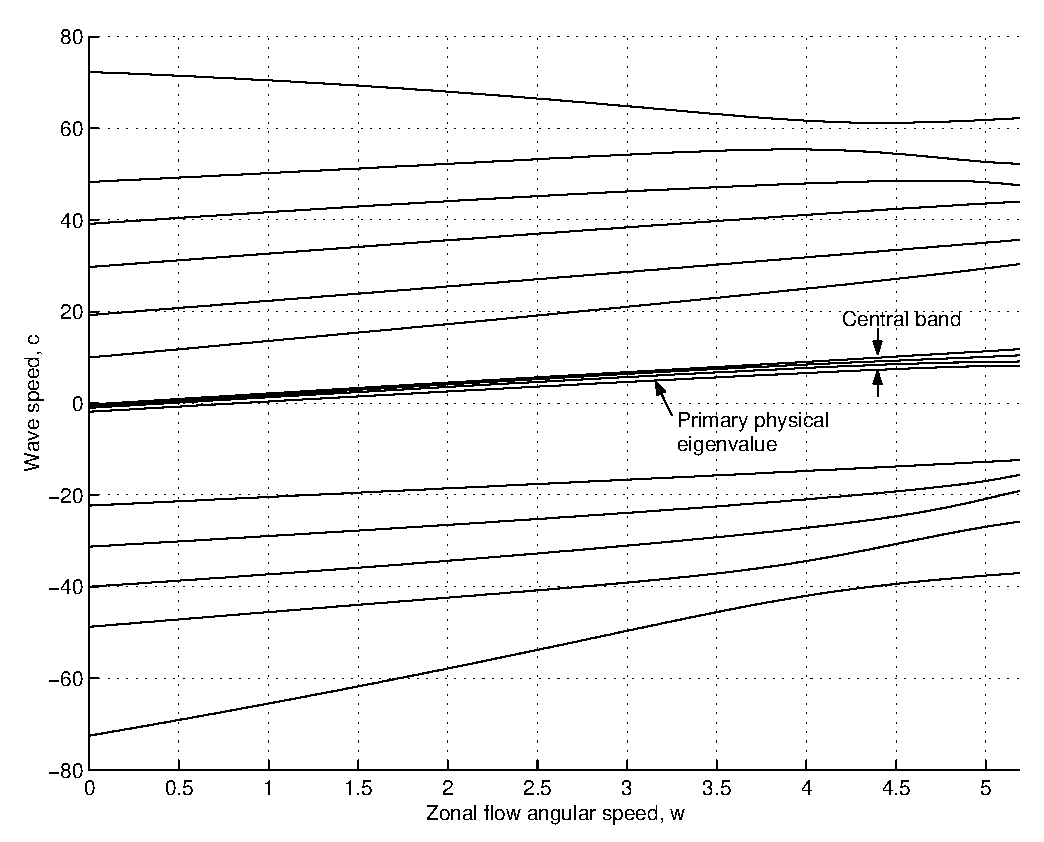
\includegraphics[scale=0.7]{IMAGES/kappa4fullspectrumN5.eps}
	\caption{Full eigen-spectrum for $\kappa=4$ with $N=5$.}
	\label{fig:wvcincompfull}
\end{figure}

It is evident that solutions to this problem can be classified into two groups: Those in the indicated central band in Figure~\ref{fig:wvcincompfull} and those lying outside this banded region. For the latter type, there was the initial suspicion that these were truncation induced solutions only; however further investigation at larger truncation levels revealed their persistence and convergence. The particular eigenvalues associated with these solutions are meaningless in a physical interpretation sense and thus can only be regarded as mathematically valid curiosities of the system. This is because the large values for the wavespeed that these solutions would imply are outside normally observed values on Earth. In addition the solutions themselves have an unphysical almost wave-less form with very little wave activity in the mid-latitudes and increased activity at the poles.
 
The \index{eigenvalues!central band}central band, on the other hand, contains much more realistic and physically meaningful solutions that demand further investigation. As labelled in Figure~\ref{fig:wvcincompfull}, we regard the banded region as consisting of a \index{eigenvalue!primary physical}primary physical eigenvalue and a series of harmonics above this base state. The primary physical eigenvalue is so labelled since it is the main solution of the system and corresponds to Rossby waves in the sense of a well defined wave structure and wavespeed.

As the truncation level is increased it is observed that this central banded region becomes more heavily populated, with higher order solutions converging to an upper limit as indicated in Figure~\ref{fig:wvcincompzoom}. While this behaviour is interesting in its own right, it is of little concern to us since the wavespeeds associated with such solutions are again rather too large to be considered as valid physical possibilities with reference to the Earth's atmosphere, where such speeds are never observed. We therefore restrict the rest of the discussion to an analysis of the primary physical eigenvalue and its main defining properties. 
\begin{figure}[htbp]
\psfrag{Zonal flow angular speed, w}{\scriptsize Zonal flow angular speed, $\omega$}
\psfrag{Wave speed, c}{\scriptsize Wavespeed, $c$}
%\psfrag{R-H solutions}{\scriptsize R-H solutions}
	\centering
		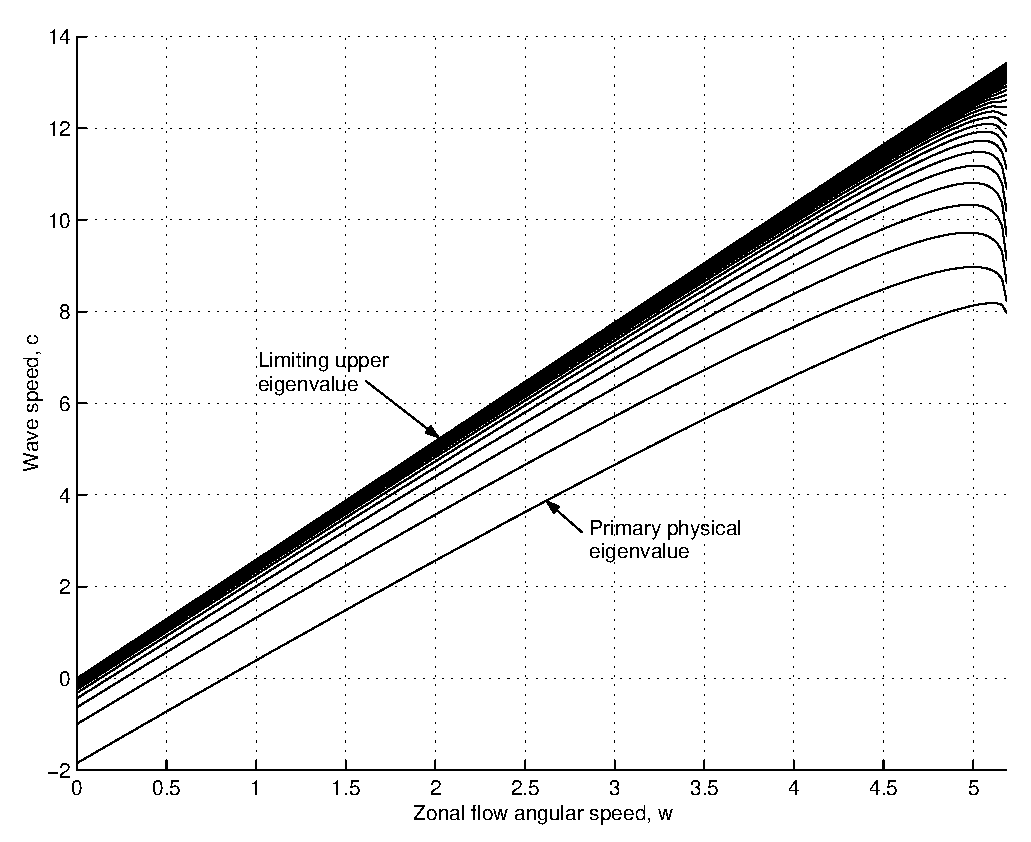
\includegraphics[scale=0.7]{IMAGES/kappa4zoomspectrumN50.eps}
	\caption{Zoomed eigen-spectrum for $\kappa=4$ with $N=50$.}
	\label{fig:wvcincompzoom}
\end{figure}

There are three main points to be made concerning Figure~\ref{fig:wvcincompzoom}. First and foremost we note that for values of $\omega$ away from the end points the wavespeed and $\omega$ relationship is close to linear. Secondly, there is a value of $\omega$ for which $c=0$ so that the linearized Rossby wave structure remains \index{Rossby wave!stationary}stationary relative to the Earth's surface. For values of $\omega$ below this critical value we have wave motion towards the west whereas for values higher we have eastward wave motion, allowing for a wide variety of atmospheric configurations. The final point concerns the behaviour at the upper end of the graph, in which no real confidence can be placed. The bending over of the solutions for large values of $\omega$ is a consequence of the fact that the height at the poles, $h_o$, is changing to conserve the total volume as previously discussed. At the other end of the graph, when $\omega=0$, we observe that the linearized solution predicts that waves with non-zero wavespeed are possible when there is no zonal flow structure. One way to interpret this behaviour is through the idea that the perturbations themselves are valid solutions of the system and that no zonal flow is required for them to exist; this idea is expanded by Pedlosky~\cite[pages 108--110]{Pedlosky:GFD}. Nonetheless, the solutions associated with values of $\omega$ away from the end points are physically reasonable, relevant and consistent with the Rossby-Haurwitz solutions, to be discussed in the next section.

\subsection{Comparison with Rossby-Haurwitz solution}
\label{subsec:rhandlincomp}
To provide evidence supporting the accuracy of the linearized solutions computed, it is useful to make a comparison between these solutions and the equivalent corresponding Rossby--Haurwitz solutions. To do this we make use of the wavespeed formula as presented in Haurwitz's classic paper \cite{Haurwitz:MAD} and later adopted by Williamson et al. in their test set. The particular formula is given by\index{Rossby--Haurwitz!formula}
\begin{equation}
c=\frac{\kappa(3+\kappa)\omega-2\Omega}{(1+\kappa)(2+\kappa)}
\end{equation}
which has been rewritten to reflect the naming conventions and variable names used in this work. Note that this equation clearly shows a linear relationship between $c$ and $\omega$. Also, Haurwitz's work does not allow one to fix the volume for the calculation, since it does not use a free-surface formulation, so we should expect some divergence from our solutions, which do take this into account.
\begin{figure}[htbp]
\psfrag{kappa=3}{\scriptsize $\kappa=3$}
\psfrag{kappa=4}{\scriptsize $\kappa=4$}
\psfrag{kappa=5}{\scriptsize $\kappa=5$}
\psfrag{Zonal flow angular speed, w}{\scriptsize Zonal flow angular speed, $\omega$}
\psfrag{Wave speed, c}{\scriptsize Wavespeed, $c$}
%\psfrag{R-H solutions}{\scriptsize R-H solutions}
	\centering
		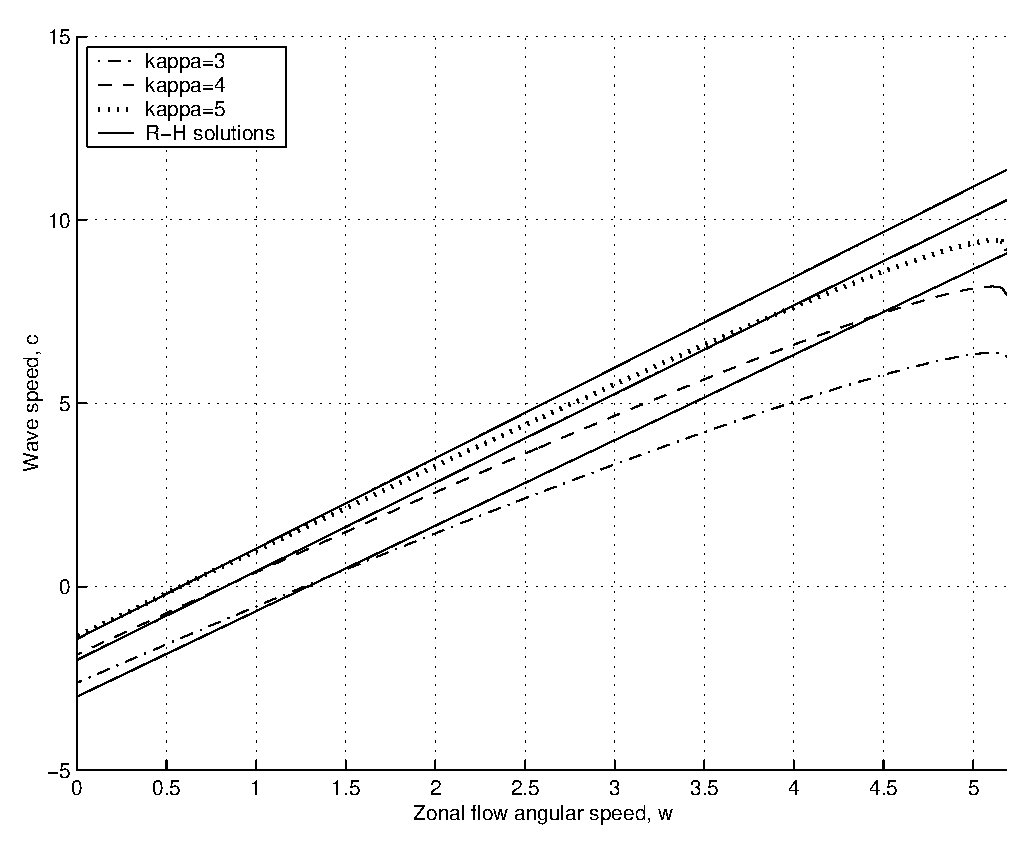
\includegraphics[scale=0.7]{IMAGES/wvchconst1.eps}
	\caption{Comparison of incompressible linearized and Rossby-Haurwitz solutions for $\kappa=3,4$ and 5 with $N=100$.}
	\label{fig:wvcincomp}
\end{figure}

To compare the two solution types we consider the primary physical eigenvalues for $\kappa=3,4$ and 5 with the equivalent Rossby-Haurwitz solutions over our valid $\omega$ range. Figure~\ref{fig:wvcincomp} shows the results of this comparison with the solid lines representing the equivalent \index{Rossby--Haurwitz!comparison with incompressible\\linearized solution}Rossby-Haurwitz solution for $\kappa=3$ to 5 from bottom to top respectively. In general one can conclude that the two models have good agreement, especially so for values of $\omega$ in the range $0<\omega<2$ where the effect of the volume matching is minimal. In fact better agreement is observed if one does not take the volume matching into consideration and fixes $h_o=1$, however the validity of the comparison between various values of $\omega$ is questionable in this case.

It is also useful to examine the resulting free-surface contours produced by both models. In order to match the height contour levels it it necessary to specify some equivalent value of the wave amplitude $\epsilon$. To make comparison possible we choose to match the two \index{height field matching}height fields at $(\eta,\phi)=(0,\pi/4)$ which represents a reasonable mid point level in each contour set. It is interesting to note that despite the fact that Haurwitz did not use a free-surface formulation, the resulting height field may be calculated via an analysis of the pressure field, as developed by Phillips\cite{Phillips:NIP}.

\begin{figure}[htbp]
	\centering
		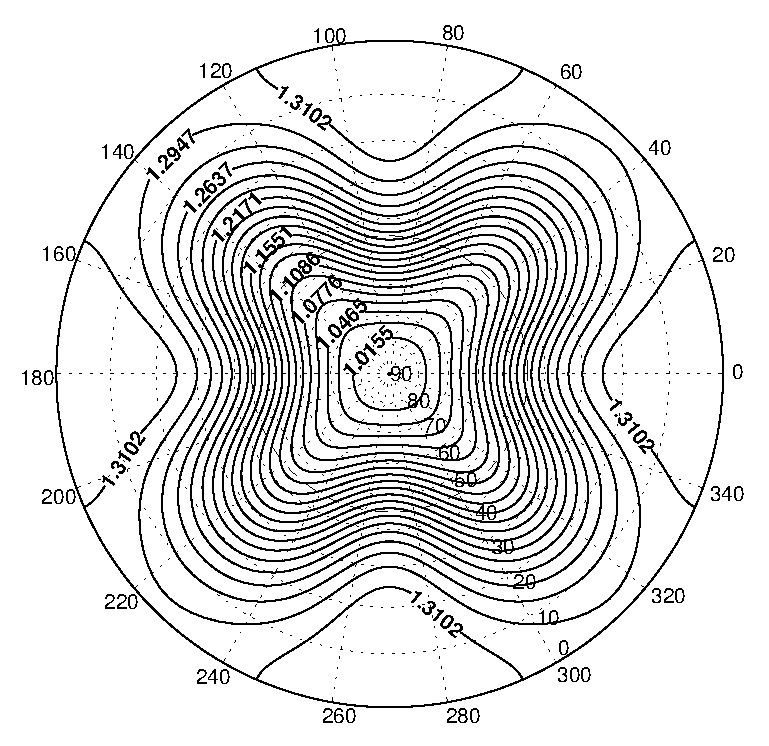
\includegraphics[scale=0.75]{IMAGES/swfsconts.eps}
	\caption{Incompresible shallow atmosphere free-surface contours for $\kappa=4$ with $N=100$.}
	\label{fig:swfsconts}
\end{figure}
\begin{figure}[htbp]
	\centering
		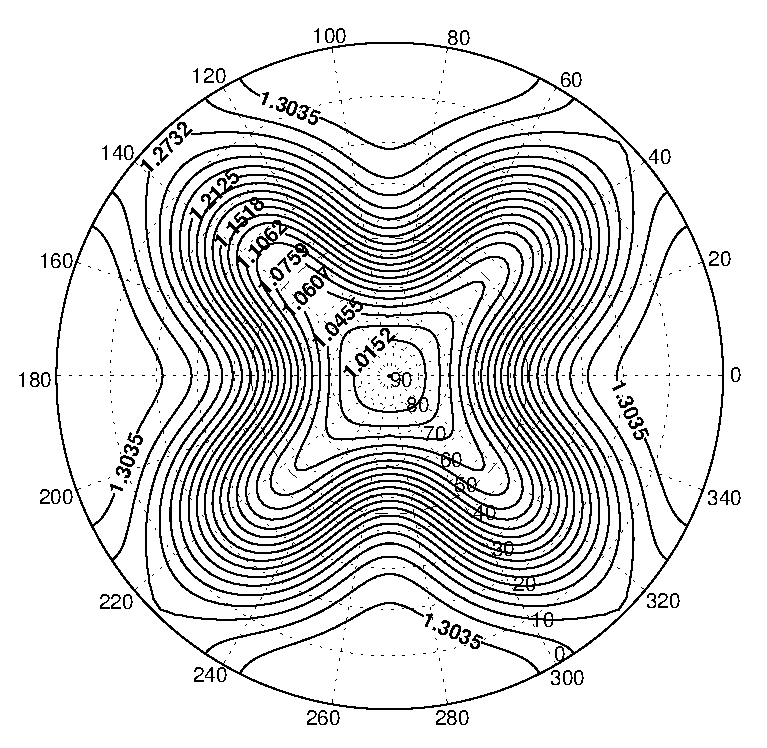
\includegraphics[scale=0.75]{IMAGES/rhfsconts.eps}
	\caption{Rossby--Haurwitz \index{Rossby--Haurwitz!free-surface contours}free-surface contours for $\kappa=4$.}
	\label{fig:rhfsconts}
\end{figure}

Figures \ref{fig:swfsconts} and \ref{fig:rhfsconts} provide a solution comparison both qualitatively, through a visual comparison, and quantitatively, through the specific contour levels of each height field. The latitudinal circle at $\phi=\pi/4$ is indicated to show where the match takes place. All plots were made using a \index{polar stereographic projection}polar stereographic projection of the Northern Hemisphere, described exhaustively in Snyder's monumental work\cite{Snyder:MP}. Of particular interest is the slight pinching of crests and troughs for the Rossby--Haurwitz wave structure that is not evident in the linearized solution. This in turn forces the lower heights, and hence pressures, near the poles to extend further towards the equator in the Rossby--Haurwitz solution. However, overall there is very close agreement between both types of solutions, encouraging one to assume that these indeed are valid approximate solutions of the full non-linear governing equations.

As a final supporting statement we investigate the nature of the corresponding velocity vector field for the free-surface presented in Figure~\ref{fig:swfsconts}. From a \index{geostrophic approximation}geostrophic point of view we would expect the fluid streamlines to be nearly parallel to the pressure contours, something which is observed in Figure~\ref{fig:fsvelfield}. Additionally we have increasingly diminishing flow as we approach either pole, which converges to the required stagnation point when $\phi=\pm \pi/2$. Since the particular viewpoint of the projection means that the sphere's rotation is counter clockwise when viewed from above, we see that fluid flow is directed in the same direction as the underlying zonal flow with the Rossby wave pattern moving relative to this mean fluid progression.
\begin{figure}[htbp]
	\centering
		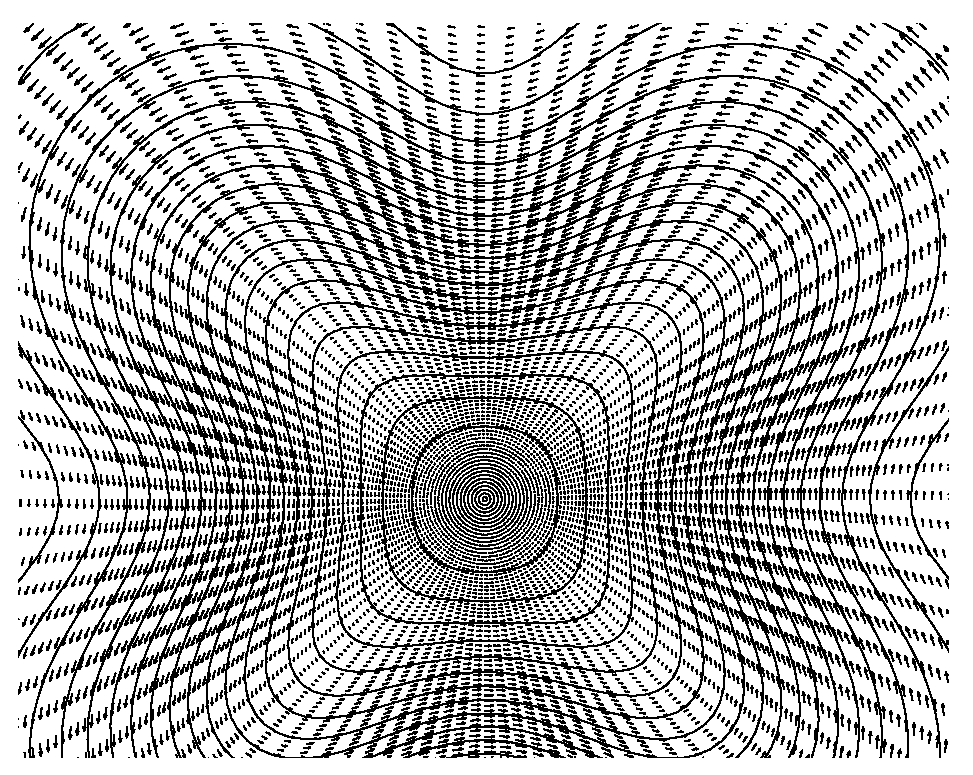
\includegraphics[scale=0.8]{IMAGES/fsvelfield.eps}
	\caption{Incompressible shallow atmosphere free-surface contours with corresponding velocity vector field for $\kappa=4$ with $N=100$}
	\label{fig:fsvelfield}
\end{figure}

In this chapter we have explored linearized solutions of the incompressible, non-dimensional shallow atmosphere equations. The solutions that were obtained for particular values of longitudinal wave number $\kappa$ were found to be in close agreement with the corresponding Rossby-Haurwitz solutions. Not only do the linearized solutions provide helpful insight into this complex dynamical system, they can also be used as a base starting point for a more thorough investigation of the complete nonlinear system. This problem is addressed in the next chapter.

